\RequirePackage{fix-cm}
\documentclass[oneside]{report}

% Biên dịch bằng XeLaTeX + BibTeX hoặc Tectonic.
\usepackage{fontspec}
\newcommand{\ThesisTitle}{Longitudinal Learning with Tensor Fusion for Predicting Progression of Alzheimer’s Disease}
\newcommand{\ThesisTitleVN}{Học dọc theo thời gian với hợp nhất tensor để dự báo tiến triển bệnh Alzheimer}
\title{\ThesisTitle}
\author{Nguyễn Phương Nam}
\date{2026}
% Cùng family và weight với bản mẫu Nguyễn Phương Trang.
% Dùng tên file OpenType từ TeX distribution, không cần cài font hệ thống.
\setmainfont{LibertinusSerif}[
  Extension=.otf,
  UprightFont=*-Regular,
  BoldFont=*-Semibold,
  ItalicFont=*-Italic,
  BoldItalicFont=*-SemiboldItalic
]
% Giữ các family Latin Modern mặc định cho sans-serif/monospace như bản mẫu.

% Cùng lề trang với bản mẫu Nguyễn Phương Trang: A4, trái 3 cm,
% phải 2 cm, trên 2 cm, dưới 2.5 cm; chữ 13 pt, giãn dòng 1.3.
\usepackage[a4paper,left=30mm,right=20mm,top=20mm,bottom=25mm]{geometry}
\usepackage{graphicx}
\graphicspath{{image/}{figures/}}
\usepackage{tikz}
\usetikzlibrary{arrows.meta,positioning,calc,fit,backgrounds,shapes.geometric,matrix}
\usepackage{xcolor}
\definecolor{uetblue}{HTML}{0B4F78}
\definecolor{softblue}{HTML}{DCEEFF}
\definecolor{softgreen}{HTML}{E2F3E7}
\definecolor{softorange}{HTML}{FCE8D5}
\definecolor{softpurple}{HTML}{EAE2F3}
\definecolor{softgray}{HTML}{F3F4F6}
\definecolor{darkgreen}{HTML}{247A3C}
\definecolor{darkorange}{HTML}{B85C00}

\usepackage{amsmath,mathtools}
\usepackage{newtxmath}
\usepackage{bm}
\usepackage{booktabs,tabularx,longtable,multirow,array}
\usepackage{float}
\usepackage{caption}
\usepackage{subcaption}
\captionsetup{font=normalsize,labelfont=normalfont,textfont=normalfont,skip=6pt}
\usepackage{enumitem}
\usepackage{listings}
\usepackage{microtype}
\usepackage{scrextend}
\usepackage{indentfirst}
\usepackage{titlesec}
\usepackage{tocloft}
\usepackage{xurl}
\usepackage{csquotes}

% Numeric citations in first-appearance order; portable XeTeX/BibTeX build.
\usepackage[numbers,sort&compress]{natbib}
\usepackage{placeins}

\usepackage{hyperref}
\hypersetup{
  colorlinks=true,
  linkcolor=blue,
  citecolor=blue,
  urlcolor=blue,
  pdftitle={\ThesisTitle},
  pdfauthor={Nguyễn Phương Nam},
  pdfsubject={Longitudinal multimodal survival prediction with RC-Free CP-factorized pairwise fusion},
  pdfkeywords={Alzheimer, MCI, longitudinal learning, tensor fusion, CP, survival analysis}
}

\changefontsizes{13pt}
\renewcommand{\baselinestretch}{1.30}
\setlength{\parindent}{1cm}
\setlength{\parskip}{5pt}
\setlist{leftmargin=1cm,itemsep=0.2em,topsep=0.3em}
\titlespacing*{\section}{0pt}{0.8\baselineskip}{0.35\baselineskip}
\titlespacing*{\subsection}{0pt}{0.65\baselineskip}{0.25\baselineskip}
\titlespacing*{\subsubsection}{0pt}{0.5\baselineskip}{0.2\baselineskip}

\titleformat{\chapter}[display]{\normalfont\bfseries\huge}{\chaptername\ \thechapter}{8pt}{\Huge}
\titlespacing*{\chapter}{0pt}{0pt}{18pt}
\renewcommand{\chaptername}{Chương}
\renewcommand{\contentsname}{MỤC LỤC}
\renewcommand{\listfigurename}{DANH MỤC HÌNH VẼ}
\renewcommand{\listtablename}{DANH MỤC BẢNG}
\renewcommand{\figurename}{Hình}
\renewcommand{\tablename}{Bảng}

\renewcommand{\cftchappresnum}{Chương~}
\renewcommand{\cftchapleader}{\normalfont\cftdotfill{\cftdotsep}}
\settowidth{\cftchapnumwidth}{Chương~10\quad}
\renewcommand{\cftfigpresnum}{Hình~}
\settowidth{\cftfignumwidth}{Hình~10.10\quad}
\renewcommand{\cfttabpresnum}{Bảng~}
\settowidth{\cfttabnumwidth}{Bảng~10.10\quad}
\settowidth{\cftsecnumwidth}{10.10\quad}
\settowidth{\cftsubsecnumwidth}{10.10.10\quad}

\newcolumntype{L}[1]{>{\raggedright\arraybackslash}p{#1}}
\newcolumntype{C}[1]{>{\centering\arraybackslash}p{#1}}
\newcolumntype{R}[1]{>{\raggedleft\arraybackslash}p{#1}}
\newcolumntype{Y}{>{\raggedright\arraybackslash}X}
\newcommand{\R}{\mathbb{R}}
\newcommand{\T}{\mathsf{T}}
\newcommand{\Had}{\odot}
\newcommand{\concat}{\mathbin{\|}}
\newcommand{\softplus}{\operatorname{softplus}}
\newcommand{\LN}{\operatorname{LN}}
\newcommand{\MLP}{\operatorname{MLP}}
\newcommand{\diag}{\operatorname{diag}}
\newcommand{\sigmoid}{\operatorname{sigmoid}}

\lstdefinestyle{pythonstyle}{
  language=Python,
  basicstyle=\ttfamily\small,
  keywordstyle=\color{uetblue}\bfseries,
  commentstyle=\color{gray},
  stringstyle=\color{darkorange},
  breaklines=true,
  frame=single,
  backgroundcolor=\color{softgray},
  columns=fullflexible,
  showstringspaces=false
}

\setlength{\emergencystretch}{2em}

\newcommand{\bestresult}[1]{\textbf{\boldmath #1}}

\providecommand{\doi}[1]{\href{https://doi.org/#1}{DOI: \nolinkurl{#1}}}
\newcommand{\thesisurl}[1]{\url{#1}}
\renewcommand{\topfraction}{0.90}
\renewcommand{\bottomfraction}{0.85}
\renewcommand{\textfraction}{0.08}
\renewcommand{\floatpagefraction}{0.72}
\setcounter{topnumber}{3}
\setcounter{bottomnumber}{2}
\setcounter{totalnumber}{5}

% The direct research baseline is deliberately bibliography item [1].
\begin{document}
\nocite{aghajanian2025longitudinal}

\hypersetup{pageanchor=false}
\begin{titlepage}
\begin{tikzpicture}[overlay,remember picture]
  \draw[line width=3pt] ($(current page.north west)+(2.0cm,-2.0cm)$) rectangle ($(current page.south east)+(-1.5cm,1.8cm)$);
  \draw[line width=1pt] ($(current page.north west)+(2.15cm,-2.15cm)$) rectangle ($(current page.south east)+(-1.65cm,1.95cm)$);
\end{tikzpicture}
\begin{center}
  \vspace*{0.1cm}
  {\large\bfseries VIETNAM NATIONAL UNIVERSITY, HANOI\\UNIVERSITY OF ENGINEERING AND TECHNOLOGY}

  \vspace{1.1cm}
  
\includegraphics[width=0.25\textwidth]{UET.png}

  \vspace{0.5cm}
  {\Large\bfseries NGUYEN PHUONG NAM}

  \vspace{1.2cm}
  {\Large\bfseries\ThesisTitle}

  \vspace{2.0cm}
  {\large\bfseries BACHELOR THESIS\\Major: Artificial Intelligence}

  \vfill
  {\large\bfseries HA NOI -- 2026}
\end{center}
\end{titlepage}

\begin{titlepage}
\begin{tikzpicture}[overlay,remember picture]
  \draw[line width=3pt] ($(current page.north west)+(2.0cm,-2.0cm)$) rectangle ($(current page.south east)+(-1.5cm,1.8cm)$);
  \draw[line width=1pt] ($(current page.north west)+(2.15cm,-2.15cm)$) rectangle ($(current page.south east)+(-1.65cm,1.95cm)$);
\end{tikzpicture}
\begin{center}
  \vspace*{0.1cm}
  {\large\bfseries ĐẠI HỌC QUỐC GIA HÀ NỘI\\TRƯỜNG ĐẠI HỌC CÔNG NGHỆ}

  \vspace{1.1cm}
  
\includegraphics[width=0.25\textwidth]{UET.png}

  \vspace{0.5cm}
  {\Large\bfseries NGUYỄN PHƯƠNG NAM}

  \vspace{1.2cm}
  {\Large\bfseries\ThesisTitle}

  \vspace{1.4cm}
  {\large\bfseries KHÓA LUẬN TỐT NGHIỆP CỬ NHÂN\\Ngành: Trí tuệ nhân tạo}

  \vspace{1.0cm}
  \begin{flushleft}
  \textbf{Sinh viên:} Nguyễn Phương Nam\quad\textbf{Mã sinh viên:} 23020406\\[0.35cm]
  \textbf{Cán bộ hướng dẫn:} GS. Nguyễn Linh Trung\\[0.35cm]
  \textbf{Cán bộ đồng hướng dẫn:} TS. Nguyễn Thành Trung
  \end{flushleft}

  \vfill
  {\large\bfseries HÀ NỘI -- 2026}
\end{center}
\end{titlepage}

\begin{titlepage}
\begin{tikzpicture}[overlay,remember picture]
  \draw[line width=3pt] ($(current page.north west)+(2.0cm,-2.0cm)$) rectangle ($(current page.south east)+(-1.5cm,1.8cm)$);
  \draw[line width=1pt] ($(current page.north west)+(2.15cm,-2.15cm)$) rectangle ($(current page.south east)+(-1.65cm,1.95cm)$);
\end{tikzpicture}
\begin{center}
  \vspace*{0.3cm}
  {\large\bfseries VIETNAM NATIONAL UNIVERSITY, HANOI\\UNIVERSITY OF ENGINEERING AND TECHNOLOGY}

  \vspace{2.2cm}
  {\Large\bfseries NGUYEN PHUONG NAM}

  \vspace{1.4cm}
  {\Large\bfseries\ThesisTitle}

  \vspace{1.5cm}
  {\large\bfseries BACHELOR THESIS\\Major: Artificial Intelligence}

  \vspace{1.2cm}
  \begin{flushleft}
  \textbf{Student ID:} 23020406\\[0.35cm]
  \textbf{Supervisor:} Prof. Nguyen Linh Trung\\[0.35cm]
  \textbf{Co-supervisor:} Dr. Nguyen Thanh Trung
  \end{flushleft}

  \vfill
  {\large\bfseries HA NOI -- 2026}
\end{center}
\end{titlepage}

\clearpage
\hypersetup{pageanchor=true}

\pagenumbering{roman}
\setcounter{page}{3}
\titleformat{name=\chapter,numberless}[display]{\normalfont\bfseries\large\filcenter}{}{0pt}{}
\chapter*{TÓM TẮT}
\addcontentsline{toc}{chapter}{TÓM TẮT}

Khóa luận \emph{\ThesisTitle} nghiên cứu dự báo tiến triển MCI dưới dạng bài toán sống còn dọc đa phương thức. Từ khung CNN--T-LSTM của Aghajanian và cộng sự, nghiên cứu phát triển lần lượt các baseline MRI, ghép nối đa phương thức, tương tác từng cặp và kiến trúc hợp nhất gọn hơn; phân rã tensor được đưa vào sau khi đánh giá chi phí của outer-product.

Cohort ADNI đã đóng băng gồm 359 người, với 106 biến cố. Ba MRI được chọn trong cửa sổ đủ điều kiện 18 tháng. MRI thứ ba xác định mốc tham chiếu dự báo; biến cố được xác định sau landmark đủ điều kiện bằng ngưỡng MMSE/CDR. Dữ liệu clinical được ghép theo ngày gần nhất trong cửa sổ $\pm90$ ngày quanh MRI, nên tính sẵn có của toàn bộ đầu vào tại mốc dự báo cần được kiểm tra riêng khi triển khai tiến cứu.

Ba tương tác MRI--Radiomics (MR), MRI--Clinical (MC) và Radiomics--Clinical (RC) ban đầu dùng outer-product và định tuyến residual có cổng động. CP sau đó tham số hóa tensor \emph{trọng số} của phép song tuyến, giữ nguyên MLP phía sau. Lõi tương tác ba cặp giảm từ 229,696 xuống 3,712 tham số; validation C-index trung bình ba seed thay đổi từ 0.8344 xuống 0.8278. Ablation dẫn đến kiến trúc RC-Free Pairwise Fusion: vẫn giữ cả ba modality nhưng chỉ duy trì MR/MC. Bốn route có sigmoid gate phụ thuộc đầu vào và scale toàn cục học được, trước T-LSTM, attention theo thời gian và Cox head.

Trên benchmark chuẩn hóa, RC-Free Pairwise Fusion đạt validation C-index $0.8347\pm0.0237$ (độ lệch chuẩn mẫu qua ba seed). Kết quả ủng hộ một kiến trúc gọn có hiệu năng cạnh tranh, chưa chứng minh ưu thế thống kê. Baseline sống còn cổ điển vẫn mạnh theo quy trình lựa chọn và quy ước concordance riêng. Kiến trúc được chọn bằng validation; việc truy cập test trong lịch sử được ghi nhận như một giới hạn. Đánh giá cuối cùng theo protocol held-out chính thức chưa được thực hiện.

\textbf{Từ khóa:} Alzheimer, MCI, MRI dọc, radiomics, hợp nhất tensor, phân rã CP, gated residual, T-LSTM, phân tích sống còn.

\chapter*{ABSTRACT}
\addcontentsline{toc}{chapter}{ABSTRACT}

This thesis, \emph{\ThesisTitle}, studies longitudinal multimodal survival prediction of MCI progression, using the CNN--T-LSTM framework of Aghajanian et al. as its baseline. MRI, concatenation and pairwise fusion models are evaluated before developing a compact CP architecture.

The frozen ADNI cohort contains 359 participants and 106 events, with three MRI visits within an 18-month eligibility window. The third MRI defines the prediction reference time; events are ascertained after the eligibility landmark using MMSE/CDR thresholds. Retrospective clinical alignment within $\pm90$ days of each MRI limits claims about prospective input availability.

MRI--Radiomics (MR), MRI--Clinical (MC) and Radiomics--Clinical (RC) interactions initially use outer products and dynamic gated residual routing. CP factorizes the bilinear \emph{weight tensor}, retaining the subsequent MLP. The three-pair interaction core falls from 229,696 to 3,712 parameters, while three-seed mean validation C-index changes from 0.8344 to 0.8278. Ablation motivates RC-Free Pairwise Fusion, which retains all modalities and only MR/MC. Its four routes use input-dependent sigmoid gates and learnable global scales, followed by T-LSTM, temporal attention and a Cox head.

RC-Free achieves standardized validation C-index $0.8347\pm0.0237$ (sample SD over three seeds). At seed 20260727, it obtains the highest ablation validation score of 0.8417 and a post-hoc test score of 0.8750; the local CNN--PCA--T-LSTM Adaptation obtains 0.6625 and 0.5379, respectively. RC-Free is selected by validation and structural simplicity, although full CP has a higher post-hoc test score. Statistical superiority is not established. Historical test access makes these test results post-hoc; independent final evaluation requires an independent cohort or a previously unused held-out dataset.

\textbf{Keywords:} Alzheimer's disease, MCI, longitudinal MRI, radiomics, tensor fusion, CP factorization, gated residual routing, T-LSTM, survival analysis.

\chapter*{LỜI CẢM ƠN}
\addcontentsline{toc}{chapter}{LỜI CẢM ƠN}

Em xin bày tỏ lòng biết ơn sâu sắc tới GS. TS. Nguyễn Linh Trung và Thượng tá, TS. Nguyễn Thành Trung, Phó Chủ nhiệm Khoa Trang bị, Bệnh viện 108. Sự định hướng tận tình, những góp ý quý báu và các trao đổi nghiêm túc của các thầy đã giúp em từng bước xác định hướng đi, hiểu rõ hơn yêu cầu khoa học của đề tài và có thêm niềm tin để kiên trì hoàn thành khóa luận.

Em xin chân thành cảm ơn Cử nhân Nguyễn Phương Trang đã luôn sẵn lòng hỗ trợ, hướng dẫn và trao đổi với em trong suốt quá trình thực hiện đề tài. Những góp ý cụ thể cùng sự đồng hành ấy đã giúp em tháo gỡ nhiều vướng mắc và tiếp thêm động lực mỗi khi công việc nghiên cứu trở nên khó khăn.

Em xin trân trọng cảm ơn ông Sepehr Aghajanian, tác giả của bài báo nền tảng được tham khảo trong khóa luận, đã dành thời gian hồi đáp email và giải đáp những câu hỏi của em. Sự cởi mở và tận tâm ấy giúp em hiểu sâu hơn công trình nghiên cứu mà mình kế thừa, đồng thời khiến em thêm trân trọng tinh thần chia sẻ trong cộng đồng khoa học.

Em biết ơn tập thể Lab Avitech đã tạo điều kiện sử dụng tài nguyên máy chủ phục vụ việc huấn luyện mô hình và thực hiện các thí nghiệm. Sự hỗ trợ thiết thực về hạ tầng tính toán đã giúp em có thể theo đuổi quá trình thực nghiệm và hoàn thành nghiên cứu.

Em xin cảm ơn các thầy cô Trường Đại học Công nghệ, Đại học Quốc gia Hà Nội đã trao cho em nền tảng kiến thức quý báu. Em cũng xin ghi nhận đóng góp của các nhà nghiên cứu, cơ sở lâm sàng, nhà tài trợ và người tham gia Alzheimer's Disease Neuroimaging Initiative (ADNI), những người đã cùng xây dựng và duy trì nguồn dữ liệu có giá trị cho nghiên cứu này.

Sau cùng, em xin gửi lời biết ơn chân thành tới gia đình và những người thân yêu vì tình thương, niềm tin và sự động viên bền bỉ. Sự ủng hộ ấy là điểm tựa giúp em vững lòng trước những thử thách và đi đến những dòng cuối cùng của khóa luận.

\chapter*{LỜI CAM ĐOAN}
\addcontentsline{toc}{chapter}{LỜI CAM ĐOAN}

Tôi cam đoan nội dung trong khóa luận này là kết quả nghiên cứu và triển khai của cá nhân tôi dưới sự hướng dẫn của các giảng viên. Các ý tưởng, công thức và kết quả từ công trình khác được trích dẫn rõ ràng trong phần tài liệu tham khảo. Dữ liệu ADNI được sử dụng theo các quy định truy cập và sử dụng dữ liệu tương ứng.

Các số liệu thực nghiệm được đối chiếu với báo cáo có cấu hình, seed, phân chia dữ liệu và provenance được lưu vết. Việc lựa chọn kiến trúc trong khóa luận dựa trên validation; các giới hạn về endpoint, thời gian đầu vào và lịch sử truy cập test được trình bày rõ. Đánh giá held-out cuối cùng theo protocol chính thức chưa được thực hiện.

\vspace{1.5cm}
\begin{flushright}
Hà Nội, năm 2026\\[1.5cm]
\textbf{Nguyễn Phương Nam}
\end{flushright}

\titleformat{name=\chapter,numberless}[display]{\normalfont\bfseries\Huge}{}{0pt}{}
\chapter*{DANH MỤC TỪ VIẾT TẮT}
\addcontentsline{toc}{chapter}{DANH MỤC TỪ VIẾT TẮT}

\begin{longtable}{L{3.2cm}L{10.5cm}}
\toprule
Từ viết tắt & Nội dung \\
\midrule
AD & Alzheimer's Disease -- bệnh Alzheimer \\
ADNI & Alzheimer's Disease Neuroimaging Initiative \\
CDR & Clinical Dementia Rating \\
C-index & Concordance index \\
CN & Cognitively Normal \\
CP & CANDECOMP/PARAFAC, còn gọi là Canonical Polyadic decomposition \\
CNN & Convolutional Neural Network \\
GLCM & Gray-Level Co-occurrence Matrix \\
GLDM & Gray-Level Dependence Matrix \\
GLRLM & Gray-Level Run Length Matrix \\
GLSZM & Gray-Level Size Zone Matrix \\
LN & Layer Normalization \\
MCI & Mild Cognitive Impairment -- suy giảm nhận thức nhẹ \\
MLP & Multi-Layer Perceptron \\
MMSE & Mini-Mental State Examination \\
MRI & Magnetic Resonance Imaging \\
NGTDM & Neighbouring Gray Tone Difference Matrix \\
PCA & Principal Component Analysis \\
PH & Proportional Hazards \\
RID & Research Identifier trong ADNI \\
T-LSTM & Time-Aware Long Short-Term Memory \\
\bottomrule
\end{longtable}


\setcounter{secnumdepth}{2}
\setcounter{tocdepth}{2}
\begingroup
\hypersetup{linkcolor=blue}
\tableofcontents
\clearpage
\listoffigures
\clearpage
\listoftables
\clearpage
\endgroup

\pagenumbering{arabic}
\setcounter{page}{1}
\chapter{Giới thiệu}
\label{chap:intro}

\section{Động lực nghiên cứu}
Khóa luận dùng nghiên cứu \emph{Longitudinal structural MRI-based deep learning and radiomics features for predicting Alzheimer's disease progression} của Aghajanian và cộng sự \cite{aghajanian2025longitudinal} làm công trình tham chiếu ban đầu để phát triển và so sánh phương pháp. Nghiên cứu đó phân tích ảnh chụp cộng hưởng từ cấu trúc T1 (MRI T1) ở nhiều thời điểm, dùng mạng nơ-ron CNN để rút đặc trưng từ ảnh, T-LSTM để xem sự thay đổi qua các lần chụp, cơ chế attention để mô hình tập trung vào thông tin quan trọng và mô hình sống còn để xếp hạng nguy cơ biến cố theo thời gian. Kết quả bài báo cho thấy việc thêm radiomics chưa giúp mô hình tốt lên một cách ổn định; vì vậy, khóa luận kiểm tra xem ảnh MRI, các đặc trưng số mô tả ảnh và thông tin lâm sàng nên được kết hợp với nhau như thế nào.

Bệnh Alzheimer (Alzheimer's disease -- AD) có thể làm trí nhớ, khả năng suy nghĩ và sinh hoạt hằng ngày suy giảm dần. Suy giảm nhận thức nhẹ (Mild Cognitive Impairment -- MCI) là tình trạng cần được theo dõi, bởi những người có cùng chẩn đoán ban đầu vẫn có thể diễn biến khác nhau: một số tiến triển thành sa sút trí tuệ, một số ổn định, còn một số cải thiện \cite{petersen2018mci,jack2018niaaa}. Vì thế, nhận biết người bệnh đang ở tình trạng nào và dự báo họ có thể diễn biến ra sao là hai việc khác nhau; khóa luận tập trung vào việc thứ hai, tức là dùng thông tin đã thu thập qua các lần khám để xếp hạng người nào có nguy cơ tiến triển sớm hơn.

Khi theo dõi một người qua nhiều lần khám, ta có thể xem cả tình trạng của họ lẫn những thay đổi xảy ra theo thời gian. MRI cấu trúc cho thấy hình ảnh giải phẫu não; radiomics chuyển hình dạng, độ sáng và kết cấu của ảnh thành các đặc trưng có thể đo lường; còn các thông tin lâm sàng mô tả khả năng nhận thức và sinh hoạt \cite{vangriethuysen2017computational}. Khi được ghép đúng cách, các nguồn thông tin này có thể bổ sung cho nhau, nhưng chúng cũng có thể lặp lại cùng một thông tin, khác thang đo hoặc chứa nhiễu; do đó, khóa luận kiểm tra lợi ích của việc kết hợp dữ liệu bằng thực nghiệm thay vì mặc định rằng càng có nhiều đầu vào thì mô hình càng tốt.

\section{Phát biểu bài toán}
Đề tài \emph{Longitudinal Learning with Tensor Fusion for Predicting Progression of Alzheimer's Disease} xây dựng mô hình dự báo nguy cơ tiến triển cho nhóm người bị MCI trong dữ liệu của Alzheimer's Disease Neuroimaging Initiative (ADNI) \cite{weiner2015impact}. Mỗi người có ba lần chụp MRI được chọn trong 18 tháng đầu kể từ lần khám ban đầu, cùng các đặc trưng radiomics và thông tin lâm sàng được ghép với từng lần chụp. Mô hình đưa ra một điểm nguy cơ liên tục: điểm càng cao thì nguy cơ tương đối theo mô hình càng lớn, nhưng đây không phải phần trăm khả năng mắc AD và cũng không phải chẩn đoán AD.

\begin{figure}[htbp]
\centering
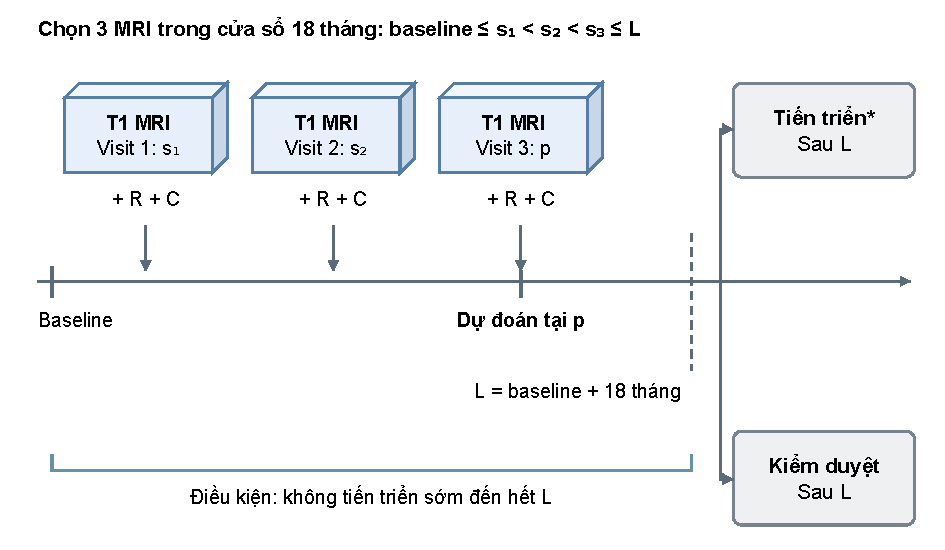
\includegraphics[width=\textwidth]{image/mci-progression-timeline.pdf}
\caption[Bài toán dự báo tiến triển MCI theo thời gian]{Sơ đồ chọn ba lần chụp MRI trong 18 tháng kể từ lần khám ban đầu. $L$ là ngày kết thúc khoảng thời gian này, bằng ngày khám ban đầu cộng 18 tháng theo lịch; đây là mốc quyết định người bệnh có được chọn vào nhóm nghiên cứu hay không. $p$ là ngày chụp MRI thứ ba và là mốc bắt đầu tính thời gian đến biến cố, nên $p\leq L$. Sau $L$, biến cố được ghi nhận khi MMSE $<24$ hoặc CDR-global $\geq1$; đây là tiêu chí dựa trên ngưỡng điểm, không phải chẩn đoán AD đã được xác nhận. $o$ là ngày xảy ra biến cố hoặc ngày theo dõi hợp lệ cuối cùng, và số năm theo dõi được tính bằng số ngày từ $p$ đến $o$ chia cho 365.25. Thông tin lâm sàng được ghép từ lần đo gần nhất trong vòng 90 ngày trước hoặc sau ngày MRI, nên đôi khi được thu thập sau khi chụp ảnh.}
\label{fig:problem-timeline}
\end{figure}

Hình~\ref{fig:problem-timeline} có hai mốc cần phân biệt. $L$ là ngày khép lại khoảng 18 tháng dùng để chọn nhóm nghiên cứu, còn $p$ là ngày chụp MRI thứ ba và là điểm bắt đầu tính thời gian đến biến cố; trong bộ dữ liệu này, $p\leq L$. Nói cách khác, $L$ quyết định ai được đưa vào nhóm nghiên cứu, còn $p$ cho biết mô hình bắt đầu tính thời gian từ ngày nào. Sau $L$, biến cố được ghi nhận ở lần đầu tiên người bệnh có MMSE $<24$ hoặc CDR-global $\geq1$; đây là \emph{dấu hiệu thay thế dựa trên điểm số}, chứ không khẳng định người đó đã được chẩn đoán AD hoặc đã được xác nhận bệnh bằng dấu ấn sinh học. Nếu người bệnh đạt một trong hai ngưỡng, chỉ báo biến cố $\delta=1$; nếu họ chưa đạt ngưỡng cho đến lần theo dõi hợp lệ cuối cùng, $\delta=0$ và dữ liệu được xem là chưa ghi nhận biến cố trong thời gian theo dõi. Vì vậy, $\delta=0$ không có nghĩa là người đó sẽ không tiến triển về sau.

Khóa luận phân tích dữ liệu đã được thu thập trước đó, và thông tin lâm sàng được ghép theo ngày gần nhất trong khoảng 90 ngày trước hoặc sau mỗi lần MRI. Vì khoảng ghép kéo dài cả về trước lẫn sau, một số thông tin có thể được ghi nhận sau ngày chụp MRI thứ ba; do đó, việc chia dữ liệu theo từng người và chỉ tính các bước tiền xử lý trên tập huấn luyện giúp hạn chế lẫn thông tin giữa các nhóm, nhưng chưa chứng minh rằng mọi đầu vào đều đã có sẵn đúng tại ngày $p$ nếu áp dụng mô hình trong thực tế. Chương~\ref{chap:method} mô tả cách ghép dữ liệu, còn Chương~\ref{chap:discussion} bàn thêm giới hạn này.

Về cách kết hợp dữ liệu, concatenation chỉ nối các nhóm đặc trưng cạnh nhau rồi để các lớp tiếp theo tự học mối liên hệ; còn phép tích ngoài (outer product) tính trực tiếp tương tác giữa từng cặp đặc trưng, nhưng số phép tính và tham số có thể tăng nhanh \cite{zadeh2017tensor}. Vì vậy, khóa luận lần lượt kiểm tra liệu có cần tạo tương tác riêng hay không, liệu có thể dùng phương pháp CP để biểu diễn gọn phần tương tác hay không, và liệu có cần giữ tương tác trực tiếp giữa mọi cặp dữ liệu hay không.

\section{Câu hỏi nghiên cứu}
Các câu hỏi trong Bảng~\ref{tab:rq} đi theo từng bước phát triển mô hình, và mỗi câu hỏi được gắn với một phép so sánh cụ thể. Kết quả chỉ phản ánh nhóm người bệnh và cách đánh giá được dùng trong khóa luận, nên không có nghĩa là một kiến trúc sẽ luôn tốt hơn trên mọi bộ dữ liệu.

Các thử nghiệm ban đầu lần lượt chuyển từ MRI đơn sang MRI theo thời gian, rồi kết hợp nhiều loại dữ liệu; tuy nhiên, trong quá trình thăm dò đó, một số phần khác như bộ trích đặc trưng, mô-đun xử lý chuỗi và cách chia batch cũng thay đổi. Vì vậy, không thể quy toàn bộ chênh lệch kết quả giữa các giai đoạn cho riêng việc thêm một loại dữ liệu hay đổi cách kết hợp; để đánh giá từng thành phần, khóa luận dựa nhiều hơn vào các phép so sánh chỉ thay đổi một yếu tố, các thử nghiệm lần lượt bỏ từng thành phần và bài đánh giá chuẩn hóa.

\begin{table}[htbp]
\centering
\caption{Câu hỏi nghiên cứu định hướng các thực nghiệm.}
\label{tab:rq}
\begin{tabularx}{\textwidth}{C{1.0cm}Y}
\toprule
\textbf{Mã} & \textbf{Câu hỏi nghiên cứu} \\
\midrule
RQ1 & Dùng nhiều lần MRI theo thời gian có giúp dự báo tốt hơn chỉ dùng MRI ở một lần khám trong nhóm nghiên cứu này không? \\
RQ2 & Khi nối các đặc trưng lại với nhau, radiomics và thông tin lâm sàng bổ sung được gì ngoài MRI? \\
RQ3 & Nếu giữ các phần khác của quy trình như nhau, tạo tương tác riêng giữa từng cặp dữ liệu có tốt hơn chỉ nối các đặc trưng không? \\
RQ4 & Dùng dạng CP để làm gọn phần tính tương tác giúp giảm số tham số đến đâu, và kết quả trên tập kiểm định thay đổi như thế nào? \\
RQ5 & Cổng điều tiết, hệ số của từng nhánh kết nối và nhánh giữ lại đặc trưng ban đầu đóng góp ra sao; có thể bỏ tương tác trực tiếp giữa radiomics và thông tin lâm sàng hay không? \\
\bottomrule
\end{tabularx}
\end{table}

\FloatBarrier
\section{Mục tiêu nghiên cứu}
Mục tiêu chung là xây dựng và phân tích một quy trình dùng nhiều lần khám cùng nhiều loại dữ liệu để dự báo tiến triển MCI, đồng thời chọn cách kết hợp dữ liệu dựa trên kết quả thử nghiệm. Cụ thể, khóa luận thực hiện các việc sau:
\begin{enumerate}
  \item Tạo nhóm người có đủ ba lần chụp MRI, xác định rõ tiêu chí ghi nhận biến cố và trường hợp chưa thấy biến cố; chia dữ liệu theo từng người và chỉ học bước chuẩn hóa từ tập huấn luyện.
  \item So sánh mô hình dùng một lần MRI, nhiều lần MRI theo thời gian và cả MRI, radiomics cùng thông tin lâm sàng để xem thời gian và mỗi loại dữ liệu bổ sung ích lợi gì.
  \item Tạo tương tác riêng giữa từng cặp MRI--radiomics, MRI--lâm sàng và radiomics--lâm sàng, rồi đưa các đặc trưng mới này trở lại mô hình bằng cơ chế điều tiết.
  \item So sánh cách tính đầy đủ các tương tác với cách biểu diễn gọn bằng CP, rồi lần lượt bỏ từng thành phần để xem thành phần nào thực sự cần thiết.
  \item Chọn mô hình dựa trên tập kiểm định, nhiều lần chạy với cách khởi tạo khác nhau và các bài đánh giá chuẩn hóa; giữ riêng tập đánh giá cuối cùng, không dùng tập này để chọn mô hình.
\end{enumerate}

\section{Đóng góp của khóa luận}
Đóng góp của khóa luận là xây dựng quy trình kết hợp dữ liệu và kiểm tra từng phần của mô hình trước khi chọn kiến trúc cuối:
\begin{enumerate}
  \item Kết hợp MRI 3D, radiomics và thông tin lâm sàng qua nhiều lần khám; T-LSTM theo dõi thay đổi theo thời gian, attention nhấn mạnh thông tin quan trọng, còn mô hình Cox dùng để xếp hạng nguy cơ biến cố.
  \item Tạo tương tác cho từng cặp dữ liệu, rồi đưa chúng trở lại mô hình qua cổng điều tiết phụ thuộc đầu vào và hệ số riêng cho mỗi nhánh. Ý tưởng có tham khảo các nghiên cứu về dùng cổng để giữ thông tin cũ và điều chỉnh mức đóng góp của thông tin mới, còn công thức cụ thể do khóa luận xây dựng \cite{ryumina2026residual,liu2026motion}.
  \item Dùng phương pháp CP, tức cách biểu diễn khối hệ số nhiều chiều (tensor trọng số) bằng các phần gọn hơn, để giảm số hệ số của lớp tương tác; cách này không phân rã dữ liệu của từng người bệnh.
  \item Chọn \textbf{RC-Free Pairwise Fusion} sau khi lần lượt bỏ từng thành phần để so sánh. Mô hình vẫn dùng đủ MRI, radiomics và thông tin lâm sàng, nhưng không tạo tương tác trực tiếp giữa radiomics và lâm sàng.
  \item So sánh các mô hình trên cùng cách chia dữ liệu qua ba lần chạy, rồi xem độ dao động kết quả và số tham số để cân nhắc giữa độ phức tạp với hiệu quả dự báo.
\end{enumerate}

CP được chọn sau khi so sánh, còn RC-Free được giữ lại sau khi thử bỏ từng thành phần và đối chiếu validation qua ba seed. Khóa luận báo cáo thêm test hậu nghiệm của các checkpoint đã chọn; các kết quả phản ánh nhóm nghiên cứu hiện tại, còn đánh giá cuối cùng trên cohort độc lập hoặc tập giữ lại mới chưa được thực hiện.

\section{Cấu trúc khóa luận}
Khóa luận gồm năm chương: Chương~\ref{chap:background} trình bày kiến thức nền về dự báo MCI, thời gian đến biến cố và kết hợp dữ liệu; Chương~\ref{chap:method} mô tả cách chọn người tham gia, xử lý dữ liệu và xây dựng mô hình. Chương~\ref{chap:results} trình bày các thí nghiệm và kết quả, còn Chương~\ref{chap:discussion} bàn về ý nghĩa, giới hạn, hướng phát triển và kết luận.

\chapter{Cơ sở lý thuyết và nghiên cứu liên quan}
\label{chap:background}

\section{MCI và tiến triển Alzheimer}
MCI mô tả suy giảm nhận thức vượt mức kỳ vọng theo tuổi nhưng chưa làm mất tính độc lập như sa sút trí tuệ. Đây là trạng thái không đồng nhất về nguyên nhân và diễn biến; chỉ một phần người bệnh tiến triển sang AD \cite{petersen2018mci}. Khái niệm lâm sàng này cũng cần được phân biệt với định nghĩa AD theo các dấu ấn sinh học trong khung nghiên cứu NIA-AA \cite{jack2018niaaa}. Khóa luận dùng nhãn tiến triển vận hành của project, không coi điểm nguy cơ do mạng sinh ra là bằng chứng xác nhận bệnh lý AD.

Trong nghiên cứu tiên lượng, câu hỏi là một sự kiện sẽ được ghi nhận khi nào sau giai đoạn quan sát. Ba visit có thể cho biết cùng một đặc điểm não đang ổn định hay thay đổi; MRI, radiomics và lâm sàng cung cấp những góc nhìn khác nhau về quá trình đó. Cơ sở dữ liệu ADNI hỗ trợ khảo sát các tín hiệu hình ảnh, lâm sàng và nhận thức theo thời gian \cite{weiner2015impact}. Tuy nhiên, điều kiện phải có đủ chuỗi visit cũng làm cohort nghiên cứu khác với toàn bộ người MCI, đặc biệt với những người tiến triển sớm hoặc thiếu theo dõi.

\section{Mô hình dọc và phân tích sống còn}
\subsection{Sự kiện, kiểm duyệt và mô hình Cox}
Gọi $T_i$ là thời gian quan sát và $\delta_i\in\{0,1\}$ là chỉ báo sự kiện. Với kiểm duyệt phải, $\delta_i=0$ chỉ cho biết chưa quan sát sự kiện đến thời điểm kết thúc theo dõi. Phân tích sống còn giữ lại thông tin thời gian và trạng thái kiểm duyệt; phân loại nhị phân tại một cửa sổ cố định trả lời một câu hỏi khác.

Mô hình Cox proportional hazards biểu diễn hazard của bệnh nhân $i$ như sau \cite{cox1972regression}:
\begin{equation}
 h_i(t)=h_0(t)\exp(\eta_i),
\end{equation}
trong đó $h_0(t)$ là baseline hazard và $\eta_i$ là log-risk. DeepSurv là một ví dụ về cách dùng mạng neural để học log-risk phi tuyến trong mô hình Cox \cite{katzman2018deepsurv}. Trong khóa luận, $\eta_i$ được thay bằng đầu ra của survival head. Chỉ số này xếp hạng nguy cơ; để có xác suất tiến triển theo một thời hạn còn cần ước lượng baseline survival và đánh giá calibration.

Với risk set $\mathcal{R}(t_i)$ gồm những người còn được theo dõi tại $t_i$, trường hợp không có ties cho negative partial log-likelihood
\begin{equation}
\mathcal{L}_{\mathrm{Cox}}
=-\sum_{i:\delta_i=1}\left(\eta_i-\log\sum_{j\in\mathcal{R}(t_i)}\exp(\eta_j)\right).
\end{equation}
Các sự kiện trùng thời gian được xử lý bằng xấp xỉ Breslow \cite{breslow1974covariance}; biểu thức nhóm ties của implementation được trình bày ở Chương~\ref{chap:method}. Harrell C-index đo khả năng sắp xếp đúng thứ tự trên các cặp có thể so sánh \cite{harrell1996multivariable}. C-index đánh giá phân biệt, không tự chứng minh calibration hoặc ích lợi lâm sàng; quy tắc xử lý ties cũng cần thống nhất khi so sánh.

Landmarking là cách đặt một mốc thời gian để xét ai còn đủ điều kiện được theo dõi trước khi dự báo kết cục tiếp theo \cite{vanhouwelingen2007dynamic}. Trong khóa luận, $L$ là ngày kết thúc khoảng chọn mẫu, bằng ngày khám ban đầu cộng 18 tháng theo lịch; còn $p$ là ngày MRI thứ ba và là mốc bắt đầu tính thời gian. Chỉ những người chưa chạm ngưỡng tiến triển đến hết $L$ mới được chọn, nên kết quả phản ánh riêng nhóm này. Thông tin lâm sàng ghép trong vòng 90 ngày có thể được ghi sau MRI, vì vậy chưa chắc đã có sẵn tại ngày $p$.

\subsection{T-LSTM và attention theo visit}
Long Short-Term Memory (LSTM) dùng trạng thái bộ nhớ và các gate để tổng hợp thông tin trong chuỗi \cite{hochreiter1997lstm}; khoảng thời gian không đều giữa hai lần khám không tự được mã hóa chỉ bằng thứ tự visit. Time-Aware LSTM (T-LSTM) sử dụng $\Delta t$ để điều chỉnh một thành phần bộ nhớ theo thời gian đã trôi qua \cite{baytas2017patient}. Đây là cơ chế phù hợp với khoảng cách visit không đều; mức lợi ích so với baseline vẫn phải được kiểm tra trên dữ liệu cụ thể.

Attention tổng hợp các hidden state $h_t$ bằng trọng số học được. Khóa luận dùng một phép chấm điểm cộng theo tinh thần additive attention \cite{bahdanau2015attention}:
\begin{equation}
 e_t=\bm v^{\top}\tanh(W_h h_t+b_h),\qquad
 \alpha_t=\frac{\exp(e_t)}{\sum_k\exp(e_k)},\qquad
 z=\sum_t\alpha_t h_t.
\end{equation}
Trọng số $\alpha_t$ mô tả cách mô hình tổng hợp visit trong lần suy luận đó; bản thân chúng không đủ để suy ra tầm quan trọng nhân quả của một lần khám.

\section{Thông tin đa phương thức}
\subsection{MRI cấu trúc và biểu diễn học sâu}
Convolutional Neural Network (CNN) học bộ lọc cục bộ với trọng số dùng chung trên ảnh \cite{lecun1998gradient}. CNN 3D mở rộng phép tích chập sang ba chiều; C3D là một công trình nền tảng cho đặc trưng không gian--thời gian trong video \cite{tran2015c3d}. Với MRI thể tích, cả ba trục đều là trục không gian, còn các visit được xử lý bởi mô hình thời gian riêng. ResNet sử dụng các kết nối residual để học phần hiệu chỉnh trên một nhánh truyền thông tin gốc \cite{he2016deep}. MedicalNet/Med3D cung cấp hướng tiền huấn luyện và transfer learning cho ảnh y tế 3D \cite{chen2019med3d}. Khóa luận khảo sát các baseline MRI trước khi cố định cấu hình encoder cho các so sánh fusion có kiểm soát.

Batch normalization chuẩn hóa theo thống kê mini-batch trong backbone \cite{ioffe2015batchnorm}; layer normalization dùng thống kê trên biểu diễn của từng mẫu và được sử dụng sau hợp nhất \cite{ba2016layernorm}. ReLU \cite{nair2010rectified} và GELU \cite{hendrycks2016gelu} là các hàm kích hoạt được dùng theo từng khối của implementation. Những thành phần này hỗ trợ tối ưu, không phải các đóng góp mới của khóa luận.

\subsection{Vision Transformer và biểu diễn ảnh 3D}
Transformer sử dụng attention để học quan hệ giữa các token \cite{vaswani2017attention}. Vision Transformer (ViT) áp dụng ý tưởng này cho chuỗi patch ảnh \cite{dosovitskiy2021vit}. Khi mở rộng sang thể tích, patch có ba chiều và attention có thể liên kết những vùng xa nhau; UNETR minh họa encoder Transformer cho ảnh y tế 3D trong tác vụ segmentation \cite{hatamizadeh2022unetr}. Đây là nền tảng của hướng ViT 3D, còn khả năng tiên lượng tiến triển cần được đánh giá bằng một protocol riêng.

CrossFormer gốc học cross-scale embeddings và attention ở khoảng cách ngắn/dài trên ảnh 2D \cite{wang2022crossformer}. Các track so sánh trong project dùng bản thích nghi CrossFormer3D Tiny cho MRI thể tích. Tên này được giữ trong phần thực nghiệm để xác định đúng backbone đã khảo sát; các paper ViT và UNETR cung cấp cơ sở lý thuyết, còn encoder của kiến trúc cuối là ResNet-18 3D khởi tạo từ MedicalNet.

\subsection{Radiomics và giảm chiều}
PyRadiomics trích xuất các descriptor định lượng từ ảnh và vùng quan tâm, bao gồm hình dạng, cường độ và kết cấu \cite{vangriethuysen2017computational}. Radiomics và CNN embedding cùng bắt nguồn từ MRI nhưng dùng hai cách biểu diễn khác nhau; vì vậy chúng có thể vừa bổ sung vừa trùng lặp thông tin. Principal Component Analysis (PCA) tạo những hướng tuyến tính trực giao tối đa hóa phương sai và được dùng để giảm chiều đầu vào \cite{jolliffe2016pca}. PCA không tối ưu trực tiếp khả năng tiên lượng; số thành phần và mọi thống kê chuẩn hóa phải được fit từ training split trong quy trình đánh giá.

\subsection{Biến lâm sàng và observedness masks}
Các thước đo như MMSE và CDR cung cấp thông tin về nhận thức và mức suy giảm chức năng \cite{folstein1975mmse,morris1993cdr}. Clinical branch trong project nhận giá trị sau tiền xử lý cùng observedness masks. Mask cho phép mô hình phân biệt một giá trị được quan sát với một giá trị được điền thay thế. Tuy nhiên, mask không khắc phục sai lệch do cơ chế thiếu dữ liệu hoặc việc đo sau thời điểm dự báo; quy tắc căn chỉnh vẫn phải được báo cáo riêng.

\section{Các chiến lược hợp nhất đa phương thức}
Học đa phương thức cần phân biệt biểu diễn, căn chỉnh và hợp nhất thông tin \cite{baltrusaitis2019multimodal}. Hình~\ref{fig:fusion-taxonomy} tổ chức các lựa chọn fusion theo hai câu hỏi: tương tác được biểu diễn như thế nào và mức đóng góp được kiểm soát như thế nào. Các nhóm không loại trừ nhau; chẳng hạn một lớp song tuyến có thể dùng CP cho trọng số và gated residual cho đầu ra.

\begin{figure}[htbp]
\centering
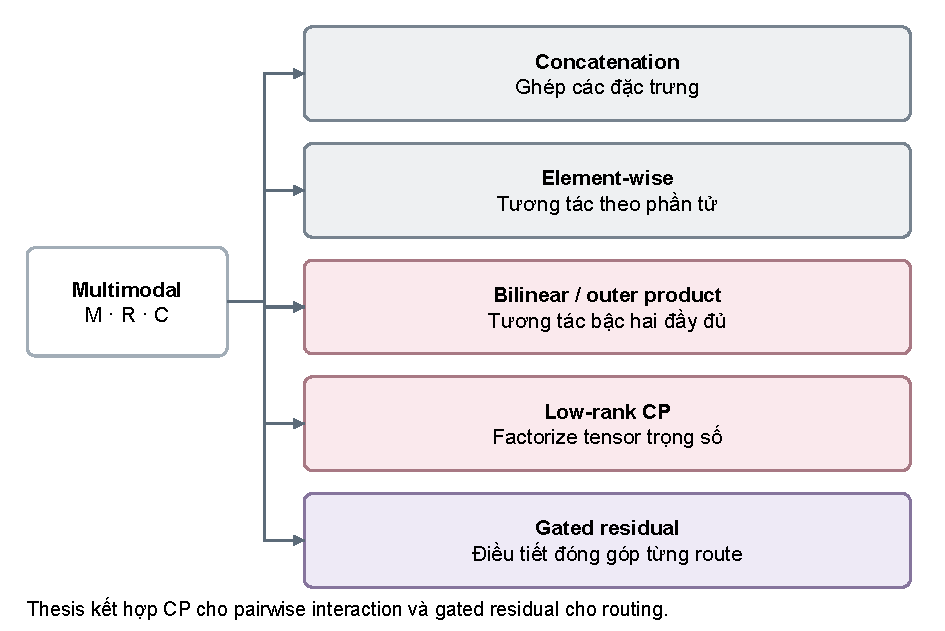
\includegraphics[width=\textwidth]{image/fusion-taxonomy.pdf}
\caption[Phân loại các chiến lược hợp nhất đa phương thức]{Các chiến lược fusion liên quan đến khóa luận. Concatenation là điểm xuất phát; bilinear/outer-product biểu diễn tương tác tường minh; low-rank factorization kiểm soát số tham số; gate và residual điều chỉnh cách bổ sung tương tác vào biểu diễn gốc. CP và gated residual là hai lựa chọn có thể kết hợp trong cùng khối fusion.}
\label{fig:fusion-taxonomy}
\end{figure}

\textbf{Concatenation} nối các vector và để MLP phía sau học quan hệ. \textbf{Tích từng phần tử} tạo tương tác đơn giản sau khi các vector được đưa về kích thước tương thích, nhưng không liệt kê đầy đủ mọi cặp chiều. \textbf{Bilinear/outer-product fusion} mô hình hóa trực tiếp tích chéo giữa các chiều; Tensor Fusion Network là một ví dụ tiêu biểu trong học đa phương thức \cite{zadeh2017tensor}. \textbf{Low-rank fusion} ràng buộc cấu trúc trọng số để giảm độ phức tạp \cite{liu2018lowrank}. \textbf{Adaptive/gated fusion} bổ sung một cơ chế chọn mức đóng góp phụ thuộc đầu vào.

Với cohort nhỏ, biểu diễn phong phú hơn cũng có thể làm tăng phương sai ước lượng. Vì vậy, trình tự của project là thiết lập concatenation, khảo sát pairwise tương tác đầy đủ, rồi mới thay lõi bằng CP và kiểm tra khả năng rút gọn topology. Đây là các giả thuyết thiết kế cần bằng chứng validation, không phải một bảng xếp hạng cố định giữa các loại fusion.

\section{Tương tác song tuyến và phân rã tensor}
Với $x\in\mathbb{R}^{d_x}$ và $y\in\mathbb{R}^{d_y}$, outer-product $xy^{\top}$ chứa mọi tích $x_i y_j$. Flatten ma trận này rồi dùng một lớp linear tương đương ánh xạ song tuyến
\begin{equation}
 h_k=\sum_{i=1}^{d_x}\sum_{j=1}^{d_y}W_{kij}x_i y_j+b_k,
\end{equation}
với tensor trọng số $W\in\mathbb{R}^{d_o\times d_x\times d_y}$. Lõi trọng số chứa $d_od_xd_y$ tham số, chưa tính bias.

CP decomposition biểu diễn tensor như tổng các tensor hạng một \cite{carroll1970candecomp,kolda2009tensor}. Áp dụng cấu trúc này cho \emph{tensor trọng số của lớp song tuyến}, với rank $Q$, cho
\begin{equation}
 W_{kij}\approx\sum_{q=1}^{Q}O_{kq}A_{iq}B_{jq},
 \qquad
 h=O\big[(A^{\top}x)\odot(B^{\top}y)\big]+b.
\end{equation}
Các factor $A$, $B$ và $O$ được học; không cần dựng outer-product tường minh. Lõi trọng số còn $Q(d_x+d_y+d_o)$ tham số. Biểu thức này là cơ sở cho phép thay thế controlled CP của khóa luận; số đếm trong implementation còn tính các bias và được báo cáo riêng ở Chương~\ref{chap:results}.

Low-rank Multimodal Fusion khai thác các factor theo phương thức \cite{liu2018lowrank}, trong khi MUTAN dùng cấu trúc Tucker cho bilinear fusion \cite{benyounes2017mutan}. Các công trình này cung cấp cơ sở về tham số hóa tensor; chúng không chứng minh trực tiếp CP sẽ cải thiện tiên lượng AD. Đặc biệt, trong mô hình của khóa luận, CP factorizes the bilinear interaction weight tensor; dữ liệu MRI/radiomics/lâm sàng của một bệnh nhân không bị phân rã CP trong forward pass.

\section{Gated residual fusion}
Ryumina và cộng sự dùng một phương thức neo, gate phụ thuộc đầu vào và residual hiệu chỉnh trong Text Residual Fusion \cite{ryumina2026residual}. Liu và cộng sự đưa skeleton vào nhánh RGB qua gated residual với hệ số scale cố định $\alpha=0.5$ \cite{liu2026motion}. Đây là hai nghiên cứu ở các tác vụ khác với tiên lượng AD, cung cấp cảm hứng thiết kế về điều tiết đóng góp và scaling.

Lấy cảm hứng từ gated residual modulation trong \cite{ryumina2026residual} và explicit residual scaling trong \cite{liu2026motion}, khóa luận xây dựng cập nhật residual riêng cho từng route:
\begin{equation}
 Z_d=\mathrm{LN}\left[U_d+\sum_{p\in\mathcal{P}(d)}
 \lambda_{p\rightarrow d}\,g_{p\rightarrow d}\,E_{p\rightarrow d}\right].
\label{eq:background-route}
\end{equation}
$U_d$ là biểu diễn gốc của phương thức đích ở không gian residual; $E_{p\rightarrow d}$ là tương tác đã chiếu về cùng không gian; $g_{p\rightarrow d}$ thay đổi theo đầu vào của bệnh nhân--visit; $\lambda_{p\rightarrow d}$ là scalar học được, dùng chung cho route qua các mẫu. Hai bài báo không đề xuất nguyên vẹn công thức này. Khóa luận thích nghi ý tưởng thành định tuyến pairwise theo đích, đồng thời thay scale cố định bằng tham số học theo route.

Identity residual giữ một đường truyền cho thông tin phương thức gốc; gate và scale kiểm soát phần hiệu chỉnh nhưng không tự bảo đảm cải thiện hiệu năng. Layer normalization \cite{ba2016layernorm} được áp dụng sau tổng residual. Dropout \cite{srivastava2014dropout} giúp regularize các MLP; tối ưu dùng AdamW \cite{loshchilov2019adamw}, phát triển từ Adam \cite{kingma2015adam} với weight decay tách khỏi cập nhật gradient. Vai trò thực nghiệm của gate, scale và residual được đánh giá bằng ablation.

\section{Các nghiên cứu liên quan}
Các công trình trong Bảng~\ref{tab:related} có sự khác biệt về cohort, thời điểm dự báo, nhãn và metric. Do đó, bảng dùng để nhận diện lựa chọn phương pháp và khoảng trống, không so sánh trực tiếp số hiệu năng giữa các bài báo với thesis.

\begin{table}[htbp]
\centering
\caption{Các nghiên cứu liên quan và vị trí của khóa luận. Hai công trình cuối có tác vụ khác với survival ranking, nhưng cung cấp góc nhìn về cấu trúc tensor và fusion thích nghi.}
\label{tab:related}
\small
\setlength{\tabcolsep}{4pt}
\begin{tabularx}{\textwidth}{L{3.5cm}L{4.1cm}Y}
\toprule
\textbf{Nghiên cứu} & \textbf{Đầu vào và tác vụ} & \textbf{Liên hệ phương pháp} \\
\midrule
\mbox{Li--Fan (2019)} \cite{li2019early} & MRI hồi hải mã baseline; nhận thức dọc một năm; tiên lượng tiến triển. & Mạng hồi tiếp kết hợp tín hiệu thời gian với MRI. \\
\mbox{Ding (2023)} \cite{ding2023progression} & Biến nhân khẩu, nhận thức và đo đạc ảnh tại năm mốc; chuyển đổi hai năm. & LSTM dọc so với random forest tại index exam. \\
\mbox{Bapat (2024)} \cite{bapat2024fouryear} & MRI 3D và nhận thức dọc; chuyển đổi trong bốn năm. & CNN 3D trích đặc trưng, concatenation rồi CNN 1D. \\
\mbox{Aghajanian (2025)} \cite{aghajanian2025longitudinal} & MRI T1 dọc và radiomics; mô hình sống còn. & CNN--T-LSTM--attention; nguồn baseline trực tiếp của project. \\
\mbox{Zhang (2023)} \cite{zhang2023explainable} & Đặc điểm cấu trúc não dọc; dự báo MMSE/ADAS-Cog. & Tensor multi-task và ensemble; khác CP trọng số pairwise. \\
\mbox{Li (2026)} \cite{li2026longitudinal} & sMRI và clinical dọc; phân loại NC/MCI/AD. & Brain latent diffusion và MoE điều tiết các biểu diễn. \\
\bottomrule
\end{tabularx}
\end{table}

Aghajanian và cộng sự sử dụng 228 người MCI, mỗi người có ba MRI T1 trong 18 tháng; chuỗi CNN embedding được đưa vào T-LSTM có attention. Radiomics không cải thiện nhất quán, và thảo luận của bài báo lưu ý vai trò của huấn luyện hai bước và ensemble \cite{aghajanian2025longitudinal}. Vì vậy, khi chuyển ý tưởng vào project hiện tại, cần phân biệt lợi ích của thông tin dọc với lợi ích của encoder, quy trình huấn luyện và cơ chế fusion.

Zhang và cộng sự dự báo điểm nhận thức bằng tensor multi-task learning và ensemble \cite{zhang2023explainable}; công trình này giúp hình thành ý tưởng dùng cấu trúc tensor trong giai đoạn tìm hiểu. Khóa luận sau đó chuyển trọng tâm sang CP cho \emph{trọng số} tương tác song tuyến trong pipeline sống còn. Li và cộng sự dùng MoE cho phân loại trạng thái chẩn đoán \cite{li2026longitudinal}; cơ chế thích nghi có liên hệ với fusion, nhưng tác vụ này không tương đương với dự báo thời gian tiến triển.

\section{Khoảng trống nghiên cứu}
Khóa luận đặt ba câu hỏi trong cohort và pipeline hiện tại: tương tác tường minh bổ sung gì cho concatenation; CP có giữ hiệu năng hữu ích khi chỉ thay lõi bilinear và giữ các khối khác; và cặp trực tiếp nào cần giữ sau factorization? Chương tiếp theo triển khai kiến trúc và residual routing thích nghi; các so sánh có kiểm soát cùng validation ở Chương~\ref{chap:results} kiểm tra các giả thuyết này.

\chapter{Phương pháp}
\label{chap:method}

Chương này trình bày cách xây dựng mẫu nghiên cứu, quá trình phát triển kiến trúc và hoạt động của mô hình cuối. Ký hiệu $M$, $R$ và $C$ lần lượt chỉ embedding MRI, radiomics và clinical tại một visit. Các khối fusion được dùng chung giữa ba visits; mô hình thời gian sau đó tổng hợp chuỗi thành một điểm nguy cơ ở cấp bệnh nhân. Kết quả dùng để đánh giá các quyết định thiết kế được trình bày riêng ở Chương~\ref{chap:results}.

\section{Thiết kế nghiên cứu và xây dựng dữ liệu}
\label{sec:study-design}

\subsection{Tiêu chí chọn mẫu và ba visits}
Dữ liệu được lấy từ Alzheimer's Disease Neuroimaging Initiative (ADNI), một nghiên cứu dọc đa trung tâm về suy giảm nhận thức và AD \cite{weiner2015impact,jack2008adnimri}. Pipeline liên kết định danh bệnh nhân PTID--RID và chọn baseline MCI sớm nhất có ngày hợp lệ, mã diagnosis bằng 2 và visit code \texttt{bl} trong ADNI1, ADNIGO hoặc ADNI2. Với bệnh nhân $i$, đặt $b_i$ là ngày baseline và $L_i=b_i+18$ tháng lịch là \emph{mốc xét điều kiện cohort}.

Bệnh nhân bị loại nếu có diagnosis AD trong DXSUM, MMSE $<24$ hoặc CDR-global $\geq1$ tại hoặc trước $L_i$. Sau $L_i$, cần ít nhất một đánh giá MMSE/CDR hợp lệ để xác định event hoặc censoring. Đây là một cohort được xây dựng hồi cứu và điều kiện hóa trên việc chưa tiến triển qua cửa sổ 18 tháng; nó không đại diện cho mọi bệnh nhân MCI tại baseline.

MRI được chọn trong khoảng $[b_i,L_i]$. Các scan gần nhau được nhóm thành timepoint theo cửa sổ hai tháng tính từ scan đầu nhóm. Trong mỗi nhóm, scan primary được ưu tiên trước repeat, rồi đến processing rank và image ID. Nếu có hơn ba timepoints, giữ scan đầu, scan cuối và scan trung gian gần trung điểm thời gian nhất. Metadata QC chính thức không liên kết được với image ID của danh sách MRI hiện có, nên lựa chọn sử dụng processing fallback đã ghi trong manifest. Quy trình tạo ra ba ngày MRI tăng nghiêm ngặt $s_{i1}<s_{i2}<s_{i3}\leq L_i$.

\begin{figure}[tbp]
\centering
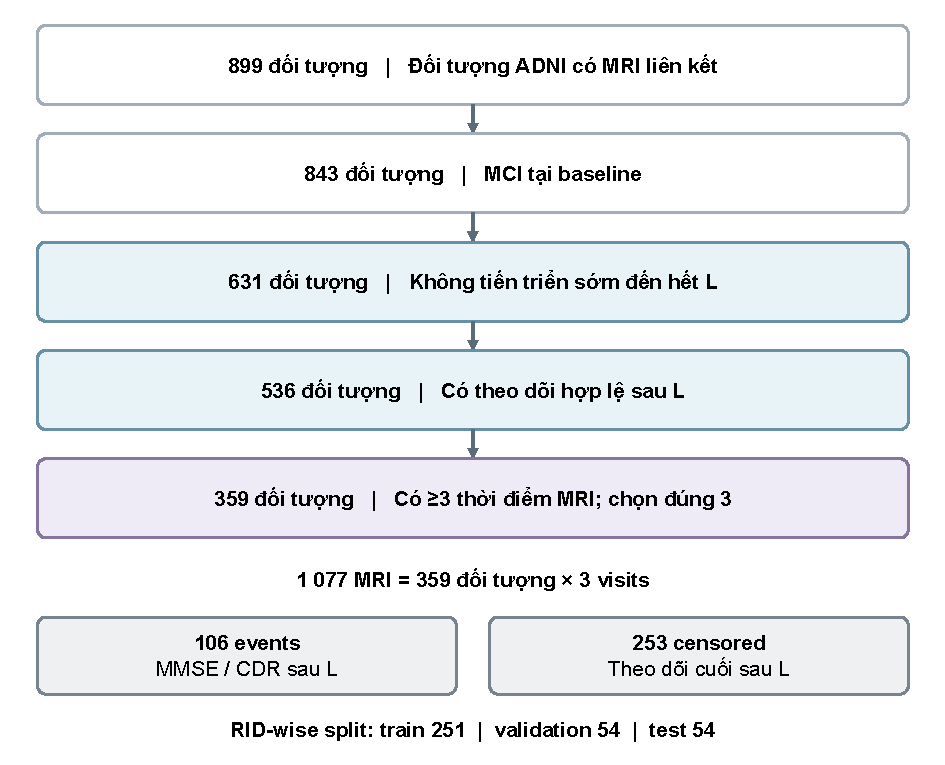
\includegraphics[width=\textwidth]{image/cohort-construction.pdf}
\caption[Quy trình xây dựng cohort dọc]{Quy trình xây dựng cohort từ metadata ADNI đến mẫu ba visits và phép chia theo RID. Số người ở các bước là số liệu của cohort đã đóng băng; MRI, radiomics và clinical được liên kết theo cùng định danh visit trước modeling.}
\label{fig:cohort}
\end{figure}

Hình~\ref{fig:cohort} tóm tắt quá trình lọc từ 899 người có MRI và liên kết định danh thành công xuống 359 người với đúng ba MRI mỗi người, tương ứng 1\,077 MRI. Cohort gồm 106 events và 253 trường hợp censored; phân bố baseline phase là ADNI1: 78, ADNIGO: 80 và ADNI2: 201. Không điều chỉnh tiêu chí để ép cỡ mẫu giống nghiên cứu tham chiếu.

\subsection{Event, censoring và mốc tính thời gian}
Sau $L_i$, event được xác định ở ngày đầu tiên có MMSE hợp lệ $<24$ hoặc CDR-global hợp lệ $\geq1$. Nếu không có event theo quy tắc này, censoring diễn ra ở ngày MMSE/CDR hợp lệ cuối cùng. Những giá trị không hợp lệ hoặc sentinel không tạo event. Endpoint này là \emph{proxy tiến triển dựa trên ngưỡng thang điểm}; nó không đòi hỏi một diagnosis AD sau $L_i$ và không xác nhận AD bằng biomarker.

Ngày tham chiếu dự báo của mô hình là $p_i=s_{i3}$, tức MRI được chọn cuối cùng. Nếu $o_i$ là ngày event hoặc censoring, nhãn survival là
\begin{equation}
 t_i=\frac{o_i-p_i}{365.25},\qquad
 \delta_i=\begin{cases}1,&\text{có event},\\0,&\text{censored}.\end{cases}
 \label{eq:survival-target}
\end{equation}
Do $p_i\leq L_i$, ngày MRI cuối và mốc xét điều kiện cohort không nhất thiết trùng nhau. Nhãn dùng thời gian từ $p_i$, trong khi mẫu đã được chọn với điều kiện không tiến triển đến $L_i$. Khoảng $[p_i,L_i]$ và điều kiện sống sót qua cửa sổ này phải được giữ rõ khi diễn giải, thay vì coi protocol hiện tại là một đánh giá tiến cứu cho mọi bệnh nhân ngay tại $p_i$.

\subsection{Phân chia và bảo vệ quá trình học}
Split cố định theo RID gồm 251 training, 54 validation và 54 test; mọi MRI của một người thuộc cùng một split. Số events tương ứng là 74, 16 và 16. Khóa liên kết xuyên modality là $(\mathrm{RID},\mathrm{visit\_index},\mathrm{image\_id},\mathrm{split})$, với kiểm tra duy nhất và bằng nhau về keyset. Imputer, scaler, loại đặc trưng hằng và PCA đều chỉ fit trên training. Diagnosis, event, ngày outcome và survival time không thuộc tập predictor.

Clinical được ghép với MRI bằng quy tắc frozen: cùng RID, đánh giá hợp lệ gần nhất trong cửa sổ \emph{$\pm90$ ngày}; hòa khoảng cách ưu tiên ngày sớm hơn rồi ID nhỏ hơn. Audit nguồn ghi nhận 294 offset MMSE/CDR dương trên các visits, với khoảng offset từ $-90$ đến $+90$ ngày. Đây là số offset đánh giá được ghép, không phải số bệnh nhân. Vì vậy, bảo vệ train-only và split không đồng nghĩa mọi predictor đã sẵn có vào ngày MRI cuối. Việc dùng clinical sau MRI trong cửa sổ ghép là giới hạn về tính khả dụng khi dự báo tiến cứu, cần kiểm tra bằng protocol chỉ dùng thông tin có trước ngày dự báo ở nghiên cứu tiếp theo.

\section{Tiền xử lý và biểu diễn từng modality}
\label{sec:preprocessing}

\begin{figure}[tbp]
\centering
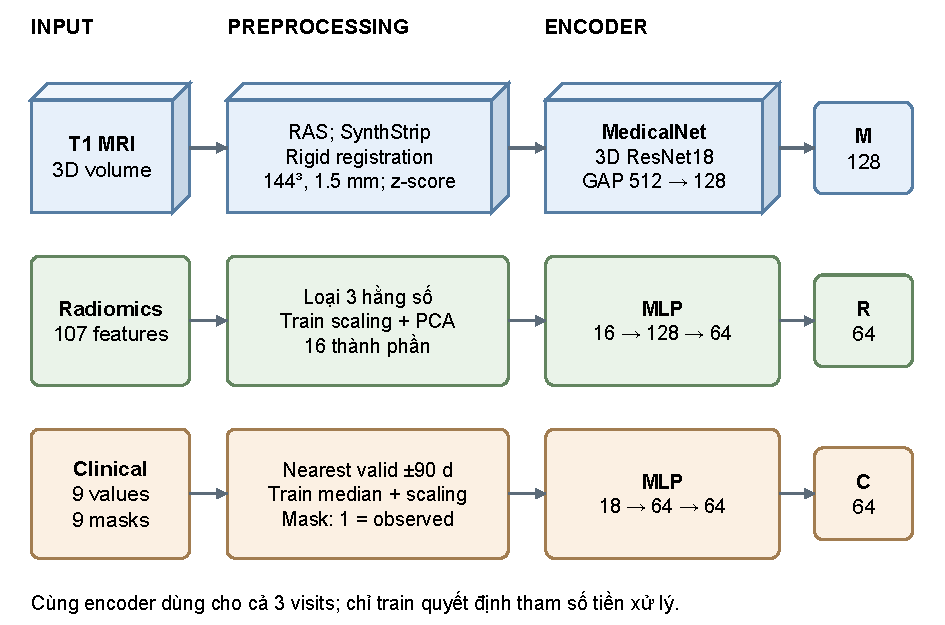
\includegraphics[width=\textwidth]{image/modality-preprocessing.pdf}
\caption[Ba nhánh xử lý modality]{Ba nhánh xử lý tại một visit. MRI tạo embedding $M$ 128 chiều; 16 thành phần radiomics PCA tạo $R$ 64 chiều; 9 giá trị clinical và 9 observedness masks tạo $C$ 64 chiều. Các biến đổi thống kê được fit trên training và giữ cố định khi áp dụng cho validation.}
\label{fig:modalities}
\end{figure}

\subsection{MRI và shared encoder}
Pipeline MRI T1 chuẩn hóa orientation RAS, dùng SynthStrip để tách não \cite{hoopes2022synthstrip}, đăng ký rigid 6-DOF các visits sau về visit đầu, rồi đăng ký rigid visit đầu về MNI152NLin2009cAsym. Ba MRI của cùng người nằm trên lưới chung $144\times144\times144$, spacing 1.5~mm isotropic. Ảnh được z-score trong brain mask riêng của volume; voxel ngoài mask bằng không. Nội suy ảnh là linear và nội suy mask là nearest-neighbor. Pipeline này không bổ sung N4, affine scaling hay nonlinear registration.

Encoder là MONAI ResNet-18 3D dùng chung trọng số giữa visits \cite{he2016deep,cardoso2022monai}. Backbone chứa BatchNorm và ReLU \cite{ioffe2015batchnorm,nair2010rectified}; sau global pooling, vector 512 chiều qua Linear $512\to128$, GELU, Dropout 0.20 và LayerNorm để tạo $M$ \cite{hendrycks2016gelu,srivastava2014dropout,ba2016layernorm}. Trong kiến trúc cuối, backbone được khởi tạo bằng MedicalNet/Med3D \cite{chen2019med3d}, nạp chặt trọng số và BatchNorm buffers của backbone, loại task head pretrained và fine-tune toàn bộ từ epoch đầu. Các mô hình MRI random và pretrained thuộc giai đoạn đối chứng, không phải hai encoder đồng thời trong pipeline cuối.

\subsection{Radiomics}
PyRadiomics trích 107 đặc trưng whole-brain từ MRI đã xử lý và mask, gồm shape, first-order, GLCM, GLDM, GLRLM, GLSZM và NGTDM \cite{vangriethuysen2017computational}. Protocol deep dùng binCount 64. Ba đặc trưng hằng trên training được loại bỏ, còn 104; scaling và PCA giữ ít nhất 99\% phương sai chỉ fit trên training \cite{jolliffe2016pca}. Dữ liệu model-ready có 16 thành phần PCA mỗi visit. Đây là chiều \emph{đầu vào} radiomics; embedding $R$ có 64 chiều sau MLP $16\to128\to64$, GELU, Dropout 0.20 và LayerNorm cuối nhánh.

\subsection{Clinical và observedness masks}
Chín predictor gồm MMSE-total, CDR-global, CDR-sum-of-boxes và sáu miền CDR: memory, orientation, judgment, community affairs, home/hobbies và personal care \cite{folstein1975mmse,morris1993cdr}. Giá trị thiếu được điền bằng median training của visit tương ứng, với median training tổng thể làm fallback, sau đó chuẩn hóa bằng mean và độ lệch chuẩn training. Chín masks riêng dùng $1$ cho giá trị quan sát được, $0$ cho giá trị thiếu. Ghép giá trị và masks tạo 18 đầu vào cho MLP $18\to64\to64$, GELU, Dropout 0.10 và LayerNorm, sinh $C\in\mathbb R^{64}$. Mask giúp phân biệt quan sát thật với giá trị điền; nó không loại bỏ giới hạn của cửa sổ ghép ngày đã nêu ở Mục~\ref{sec:study-design}.

\subsection{Thư viện và triển khai}
Các mô hình neural được triển khai bằng Python và PyTorch cho tensor, automatic differentiation, tối ưu và huấn luyện trên GPU \cite{paszke2019pytorch}. MONAI cung cấp backbone ResNet 3D cho ảnh y tế \cite{cardoso2022monai}. NumPy xử lý mảng số \cite{harris2020numpy}; pandas phục vụ đọc, ghép và kiểm tra các bảng manifest theo bệnh nhân--visit \cite{mckinney2010pandas}. NiBabel đọc volume NIfTI và thông tin affine trong các loader MRI.

Tiền xử lý dữ liệu bảng dùng scikit-learn cho scaling và PCA \cite{pedregosa2011sklearn}; PyRadiomics trích các descriptor đã nêu ở trên \cite{vangriethuysen2017computational}. Baseline Cox elastic-net, Random Survival Forest và đánh giá dữ liệu kiểm duyệt được xây dựng với scikit-survival \cite{polsterl2020sksurv}. Các script kiểm tra tiền xử lý ảnh có sử dụng Matplotlib để trực quan hóa kết quả kiểm tra \cite{hunter2007matplotlib}.

Prototype Cox ban đầu có backend TorchSurv tùy chọn \cite{monod2024torchsurv}. Các phase pairwise được đối chiếu trong khóa luận có implementation Cox/Breslow riêng, với risk set minibatch và cách xử lý ties được mô tả ở Mục~\ref{sec:training-method}. Việc trích dẫn thư viện xác định hạ tầng phương pháp; thông số của các mô hình và kết quả thực nghiệm vẫn được xác định từ artifact của từng phase.

\section{Quá trình phát triển kiến trúc}
\label{sec:architecture-evolution}
Kiến trúc được phát triển theo từng câu hỏi nghiên cứu, không bắt đầu với CP hay topology RC-Free hoàn chỉnh. MRI Only khảo sát biểu diễn không gian từ MRI cuối; Longitudinal MRI thêm T-LSTM và attention để xử lý chuỗi. Multimodal Concatenation tiếp theo kiểm tra thông tin bổ sung từ radiomics và clinical bằng phép nối đơn giản. Dynamic Pairwise Fusion đưa vào tương tác tường minh giữa từng cặp modality và định tuyến residual. Variant MedicalNet giữ cơ chế fusion nhưng thay khởi tạo backbone, sau đó trở thành reference cho thí nghiệm CP.

\begin{figure}[tbp]
\centering
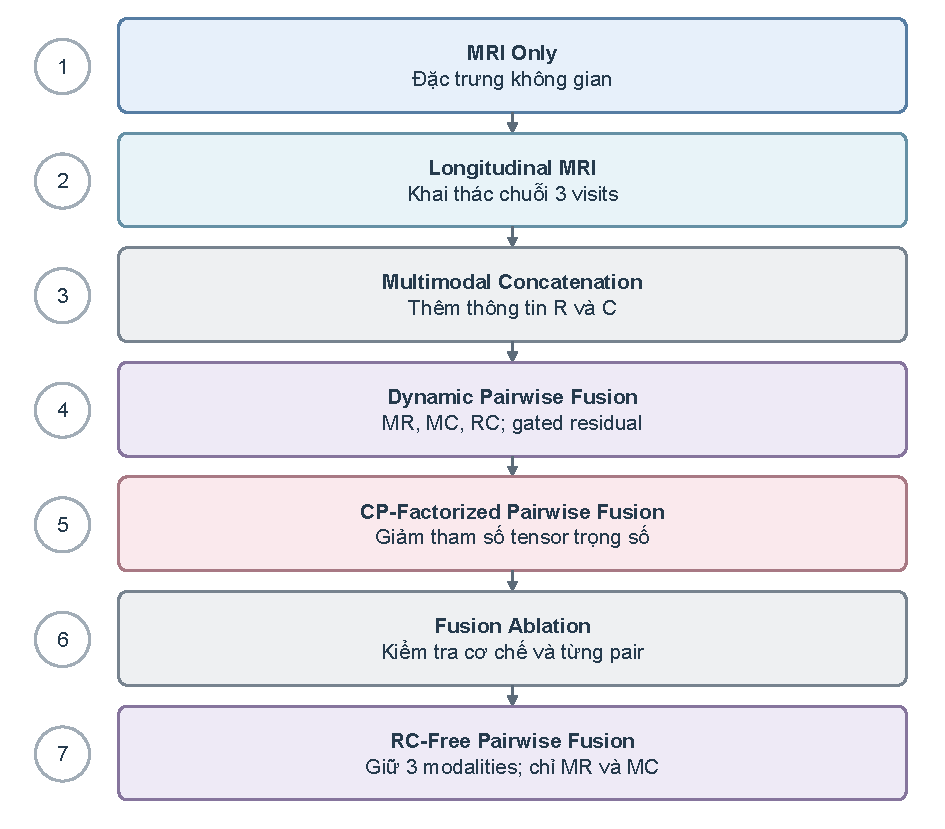
\includegraphics[width=\textwidth]{image/architecture-evolution.pdf}
\caption[Tiến hóa của framework]{Tiến hóa của framework theo các câu hỏi thực nghiệm. CP thay cách tham số hóa interaction core sau khi full outer-product đã được nghiên cứu; topology RC-Free hình thành sau fusion ablation và được kiểm tra tiếp bằng validation nhiều seed.}
\label{fig:evolution}
\end{figure}

Full outer-product tạo tương tác giàu nhưng cần lớp tuyến tính lớn. CP được áp dụng ở bước sau để giảm chi phí của lớp này trong khi giữ các khối còn lại. Fusion ablation tiếp tục kiểm tra gate, scale, identity residual và từng pair. Kết quả validation dẫn tới RC-Free Pairwise Fusion, chỉ giữ MR và MC. Hình~\ref{fig:evolution} là chronology thiết kế; các so sánh và mức độ chắc chắn của bằng chứng được trình bày ở Chương~\ref{chap:results}. Chuỗi milestone ban đầu có khác biệt về protocol batching, nên không được diễn giải toàn bộ thành các đối chứng chỉ thay duy nhất một thành phần.

\section{Multimodal Concatenation baseline}
Tại visit $t$, baseline nối ba embedding:
\begin{equation}
 F_t=\operatorname{Readout}(M_t\concat R_t\concat C_t),\qquad
 M_t\concat R_t\concat C_t\in\mathbb R^{256},\quad F_t\in\mathbb R^{128}.
\end{equation}
Readout gồm Linear $256\to128$, GELU, Dropout 0.20 và LayerNorm. Chuỗi ba $F_t$ đi qua temporal stack và Cox head. Baseline giữ thông tin của cả ba modality nhưng không có bilinear pair block hoặc route riêng, nên tạo mốc so sánh cho câu hỏi về cơ chế interaction.

\section{Dynamic Pairwise Fusion}
Trước khi tạo interaction, các phép chiếu tuyến tính không bias đưa embedding xuống
\begin{equation}
 \widetilde M\in\mathbb R^{32},\qquad
 \widetilde R\in\mathbb R^{32},\qquad
 \widetilde C\in\mathbb R^{16}.
\end{equation}
Những bottleneck này giảm chiều input nhưng full reference vẫn tạo outer-product tường minh. Với pair input $x\in\mathbb R^{d_x}$, $y\in\mathbb R^{d_y}$, đặt $v=\operatorname{vec}(xy^\top)$. MR dùng $1024\to128\to64$, MC dùng $512\to128\to64$, RC dùng $512\to64\to32$. Giữa hai Linear của pair có GELU và Dropout 0.10; cuối pair có LayerNorm.

\begin{figure}[tbp]
\centering
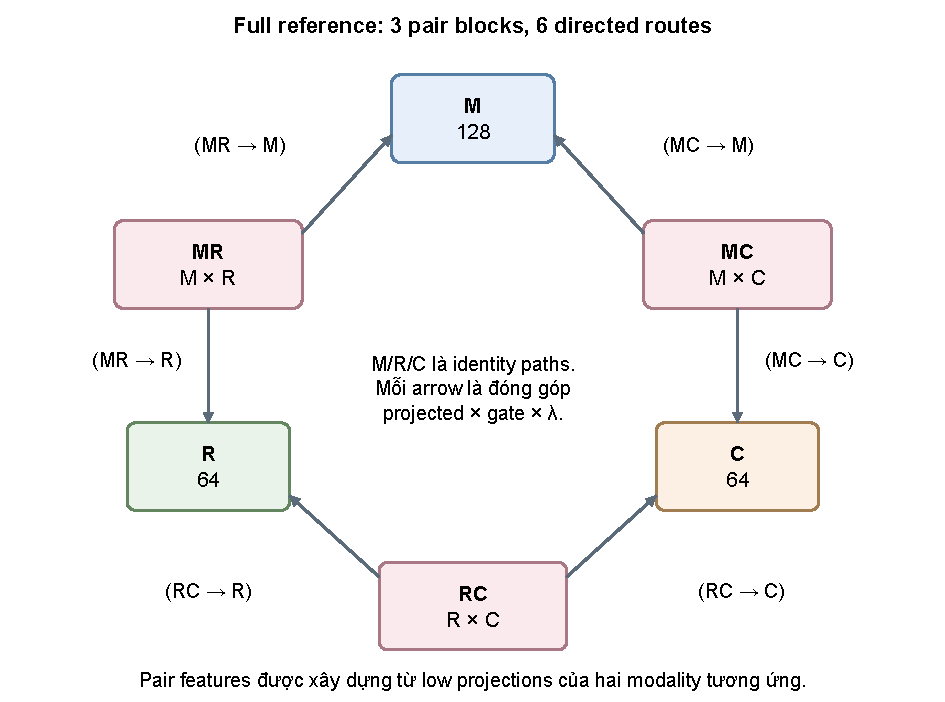
\includegraphics[width=\textwidth]{image/full-pairwise-graph.pdf}
\caption[Full pairwise graph và sáu routes]{Full pairwise graph với ba interaction MR, MC, RC và sáu directed routes về các modality thành viên. Mỗi pair chỉ được tạo một lần tại cùng patient--visit; hai hướng có adapter và gate riêng. Đây là kiến trúc reference trước khi loại RC.}
\label{fig:full-pairwise}
\end{figure}

Mỗi pair feature $E_k$ được đưa về hai modality đích bằng các adapter Linear và LayerNorm độc lập. MR và MC có feature 64 chiều, RC có feature 32 chiều. Sáu output adapter cùng chiều với modality đích: $(\mathrm{MR}\to M)$ và $(\mathrm{MC}\to M)$ là 128; $(\mathrm{MR}\to R)$, $(\mathrm{RC}\to R)$, $(\mathrm{MC}\to C)$ và $(\mathrm{RC}\to C)$ là 64. Interaction chỉ diễn ra trong một visit của một bệnh nhân, không nhân chéo người hoặc thời điểm. Hình~\ref{fig:full-pairwise} tách rõ ba pair blocks và sáu routes thay vì xem các cạnh ngược là sáu pair khác nhau.

\section{CP-factorized pairwise interaction}
\label{sec:cp-method}
Với full bilinear first layer, hidden output thứ $s$ là
\begin{equation}
 h_s=\sum_{i=1}^{d_x}\sum_{j=1}^{d_y}\mathcal W_{sij}x_i y_j+b_s,
 \qquad \mathcal W\in\mathbb R^{d_h\times d_x\times d_y}.
\end{equation}
CP tham số hóa \emph{tensor trọng số của ánh xạ bilinear}, theo dạng low-rank \cite{kolda2009tensor,liu2018lowrank}:
\begin{equation}
 \mathcal W_{sij}\approx\sum_{q=1}^{Q}O_{sq}A_{iq}B_{jq}.
 \label{eq:cp-weight}
\end{equation}
Trong mô hình này $A\in\mathbb R^{d_x\times Q}$, $B\in\mathbb R^{d_y\times Q}$ và $O\in\mathbb R^{d_h\times Q}$ được học cùng mạng. Không có bước phân rã dữ liệu bệnh nhân bằng CP. Forward tương ứng là
\begin{align}
 u&=A^\top x,\qquad v=B^\top y,\qquad q=u\odot v,\\
 h&=Oq+b,\qquad E_{xy}=\operatorname{PostMLP}_{xy}(h).
 \label{eq:cpblock}
\end{align}
$A$ và $B$ không bias; bias $b$ của first layer được giữ trong $Oq+b$. Post-MLP vẫn là GELU, Dropout 0.10, Linear $d_h\to d_o$ và LayerNorm. Vì vậy, controlled CP comparison chỉ thay first interaction transformation, giữ output shape, post-MLP, encoders, routes, gate, scale và temporal stack.

\begin{figure}[tbp]
\centering
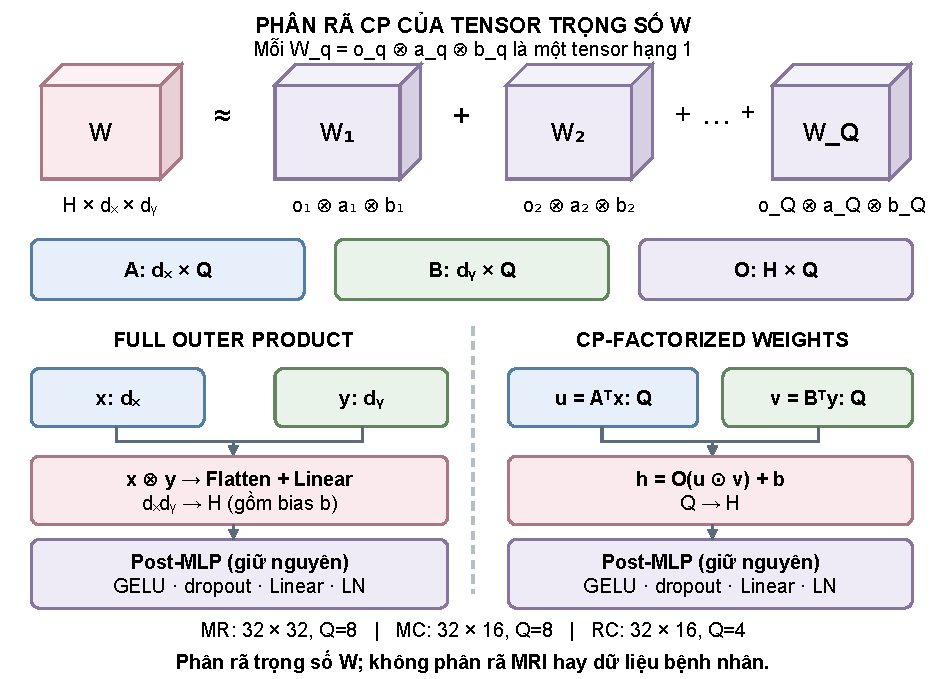
\includegraphics[width=\textwidth]{image/outer-vs-cp.pdf}
\caption[Full outer-product và CP-factorized bilinear]{Full outer-product và CP-factorized first bilinear layer. CP tính hai phép chiếu rank $Q$, tích Hadamard và phép chiếu output mà không tạo activation $d_xd_y$. Post-MLP sau first layer được giữ nguyên trong controlled comparison.}
\label{fig:cp-block}
\end{figure}

\begin{table}[H]
\centering
\caption{Cấu hình CP của full reference và kiến trúc cuối.}
\label{tab:cpconfig}
\begin{tabular}{lccccc}
\toprule
Pair & $(d_x,d_y)$ & Rank $Q$ & Hidden $d_h$ & Output $d_o$ & RC-Free \\
\midrule
MR & $(32,32)$ & 8 & 128 & 64 & Giữ \\
MC & $(32,16)$ & 8 & 128 & 64 & Giữ \\
RC & $(32,16)$ & 4 & 64 & 32 & Loại \\
\bottomrule
\end{tabular}
\end{table}

Bảng~\ref{tab:cpconfig} ghi rank thực sự được dùng; không có kết quả khảo sát rank rộng được tuyên bố trong khóa luận. First layer full có $d_hd_xd_y+d_h$ tham số; CP có $Q(d_x+d_y+d_h)+d_h$. Lợi ích trực tiếp nằm ở interaction core, trong khi backbone MRI vẫn chiếm phần lớn tổng tham số. Không suy ra mức tăng tốc toàn pipeline chỉ từ công thức tham số.

\section{Dynamic gated residual routing}
\label{sec:gated-routing}
Lấy cảm hứng từ gated residual modulation của Ryumina và cộng sự \cite{ryumina2026residual} và explicit residual scaling của Liu và cộng sự \cite{liu2026motion}, khóa luận xây dựng cập nhật residual riêng cho từng route. Hai công trình này cung cấp ý tưởng điều tiết và scaling; công thức dưới đây là thiết kế của project, không phải công thức nguyên dạng của các paper.

Với pair $k$ và modality đích $d$, ký hiệu $U_d$ là embedding modality gốc và
\begin{equation}
 \widehat E_{k\to d}=\LN_{k\to d}(W_{k\to d}E_k+b_{k\to d})
\end{equation}
là feature đã chiếu về chiều đích. Gate dùng cả trạng thái modality và feature route:
\begin{equation}
 g_{k\to d}=\sigma\!\left(
 w_{k\to d}^{\top}\operatorname{GELU}\!\left[
 V_{k\to d}\bigl(\LN_d^{\rm gate}(U_d)\concat\widehat E_{k\to d}\bigr)
 +a_{k\to d}\right]+c_{k\to d}\right).
 \label{eq:dynamic-gate}
\end{equation}
Gate MLP có hidden 32 và output một scalar trong $(0,1)$ cho mỗi patient--visit; scalar được broadcast trên các feature channels. Các routes dùng sigmoid độc lập, không cạnh tranh bằng softmax. Gate weights được khởi tạo Xavier và biases bằng không.

\begin{figure}[tbp]
\centering
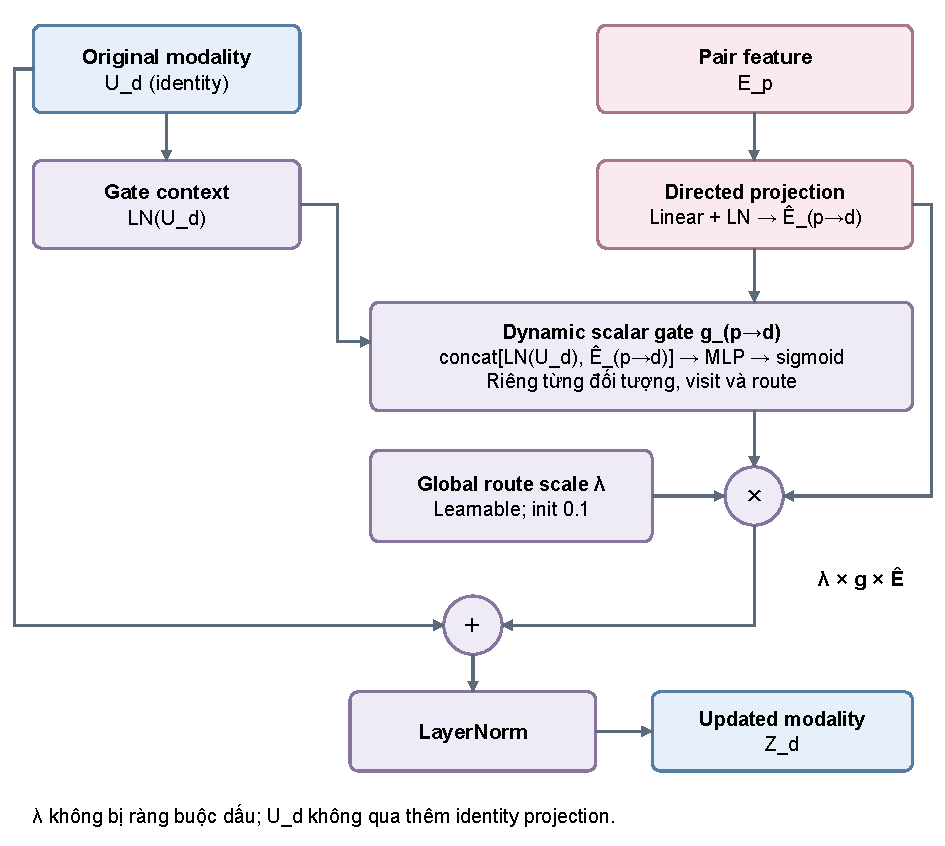
\includegraphics[width=\textwidth]{image/gated-residual-route.pdf}
\caption[Giải phẫu một gated residual route]{Giải phẫu một route: pair feature qua directed projection, nhân dynamic gate theo patient--visit và global route scale, cộng vào đường identity của modality đích rồi LayerNorm. Gate nhận modality gốc đã chuẩn hóa và directed pair feature; đường identity giữ nguyên embedding gốc trước phép cộng.}
\label{fig:route}
\end{figure}

Scale $\lambda_{k\to d}$ là scalar học được riêng cho route nhưng dùng chung giữa bệnh nhân và visits. Implementation hiện có khởi tạo $\lambda=0.1$ và \emph{không ràng buộc dấu}: đây là tham số trực tiếp, không qua softplus. Vì vậy gate biểu diễn mức điều tiết phụ thuộc input, còn $\lambda$ biểu diễn scale và dấu toàn cục của route; không đồng nhất chúng thành attention weight.

Cập nhật tổng quát của modality là
\begin{equation}
 Z_d=\LN_d^{\rm out}\left(
 U_d+\sum_{k\in\mathcal P(d)}\lambda_{k\to d}\,g_{k\to d}\,\widehat E_{k\to d}
 \right).
 \label{eq:ours-residual}
\end{equation}
$\mathcal P(d)$ là các pair còn hoạt động đi vào $d$. Đường identity dùng trực tiếp $U_d$, không thêm một phép chiếu identity học được. LayerNorm ở adapter, ở input gate và sau tổng residual là ba phép chuẩn hóa khác nhau \cite{ba2016layernorm}. Contribution thực tế phụ thuộc đồng thời $\lambda$, gate và norm feature; riêng gate hoặc scale không chứng minh ý nghĩa sinh học hay quan hệ nhân quả.

\section{RC-Free Pairwise Fusion}
\label{sec:rcfree-method}
Kiến trúc cuối cho nghiên cứu validation là RC-Free CP-Factorized Pairwise Fusion, gọi ngắn là RC-Free Pairwise Fusion. Quyết định bỏ RC được nghiên cứu sau full CP ablation rồi kiểm tra tiếp bằng nhiều seed; nó không phải giả định được áp đặt từ đầu. RC-Free loại \emph{direct radiomics--clinical pair}, đồng thời vẫn giữ cả ba unimodal branches. MRI trở thành điểm nối của hai interaction MR và MC.

Đặt $D_{k\to d}=\lambda_{k\to d}g_{k\to d}\widehat E_{k\to d}$, các output là
\begin{align}
 M_{\rm out}&=\LN_M^{\rm out}(M+D_{(\mathrm{MR}\to M)}+D_{(\mathrm{MC}\to M)}),\\
 R_{\rm out}&=\LN_R^{\rm out}(R+D_{(\mathrm{MR}\to R)}),\\
 C_{\rm out}&=\LN_C^{\rm out}(C+D_{(\mathrm{MC}\to C)}).
 \label{eq:rcfree-residual}
\end{align}

\begin{figure}[tbp]
\centering
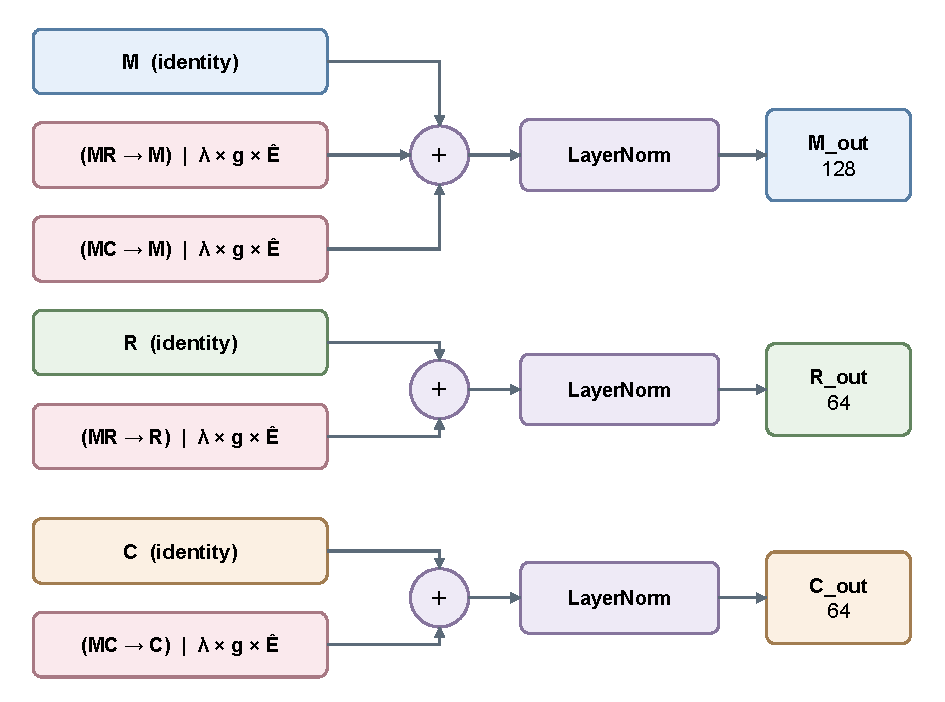
\includegraphics[width=\textwidth]{image/rc-free-routing.pdf}
\caption[Residual routing của RC-Free Pairwise Fusion]{Residual routing của RC-Free Pairwise Fusion theo ba hàng modality đích. MRI nhận MR và MC, radiomics nhận MR, clinical nhận MC. Mỗi hàng giữ đường identity, cộng contribution rồi LayerNorm; $(\mathrm{RC}\to R)$ và $(\mathrm{RC}\to C)$ không hoạt động.}
\label{fig:rcfree-routing}
\end{figure}

Hai CP blocks MR/MC dùng ranks 8/8; bốn directed adapters, bốn dynamic gates và bốn learnable scales còn hoạt động. Output vẫn là 128/64/64, nên downstream readout và temporal model không đổi. Biến thể RC-Free Fixed-$\lambda$ chỉ cố định bốn scales bằng 0.1 để khảo sát sensitivity, không thay thế kiến trúc chính. Loại một interaction không đồng nghĩa kết luận hai modality vô ích hoặc độc lập về mặt y học.

\section{Tổng quan pipeline cuối}
\label{sec:final-pipeline}
Hình~\ref{fig:overall} liên kết toàn bộ các bước. Tại mỗi visit, ba branches tạo $M_t,R_t,C_t$; hai CP pair blocks tạo MR và MC; gated residual routing tạo $M_{{\rm out},t},R_{{\rm out},t},C_{{\rm out},t}$. Phép nối giữ thứ tự MRI--radiomics--clinical, sinh 256 chiều và readout xuống $F_t\in\mathbb R^{128}$. Chuỗi $(F_1,F_2,F_3)$ cùng các khoảng cách ngày MRI đi vào T-LSTM, attention và Cox head.

\begin{figure}[tbp]
\centering
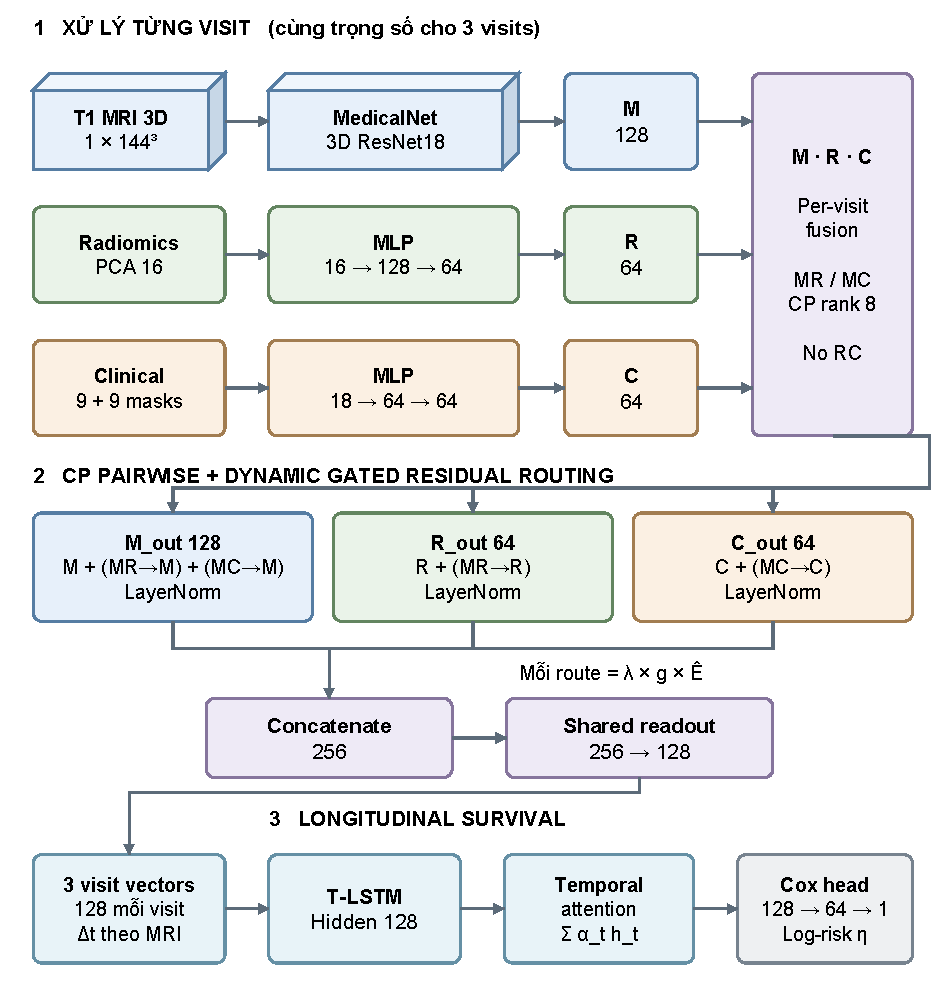
\includegraphics[width=\textwidth]{image/final-pipeline.pdf}
\caption[Kiến trúc tổng thể của framework cuối]{Kiến trúc tổng thể của Longitudinal Learning with Tensor Fusion. Phần trên xử lý một visit bằng ba encoders, CP interactions MR/MC và gated residual routing; phần dưới tổng hợp ba visit embeddings bằng T-LSTM và temporal attention, sau đó xuất raw Cox log-risk. Không có direct RC interaction trong pipeline cuối.}
\label{fig:overall}
\end{figure}

\begin{table}[H]
\centering
\caption{Kích thước tensor chính trong kiến trúc cuối, với batch size $B$.}
\label{tab:pipeline-shapes}
\begin{tabularx}{\textwidth}{Yl}
\toprule
Tensor & Shape \\
\midrule
MRI sequence & $[B,3,1,144,144,144]$ \\
Radiomics PCA & $[B,3,16]$ \\
Clinical values / observedness masks & $[B,3,9]$ / $[B,3,9]$ \\
$M_{\rm out},R_{\rm out},C_{\rm out}$ & $[B,3,128]$, $[B,3,64]$, $[B,3,64]$ \\
Readout / T-LSTM hidden sequence & $[B,3,128]$ \\
Temporal attention weights & $[B,3]$ \\
Subject embedding / raw log-risk & $[B,128]$ / $[B]$ \\
\bottomrule
\end{tabularx}
\end{table}

\section{Mô hình thời gian và temporal attention}
\label{sec:temporal-method}
T-LSTM xử lý khoảng cách visit không đều qua sự suy giảm short-term memory \cite{baytas2017patient,aghajanian2025longitudinal}. Khoảng thời gian đầu bằng không; các khoảng còn lại là $\Delta t_t=(s_t-s_{t-1})/365.25$, đo bằng năm. Không dùng số thứ tự visit thay cho khoảng ngày và không thêm learned time embedding.

Từ memory trước đó $c_{t-1}$, cell phân tách và điều chỉnh:
\begin{align}
 c_{t-1}^{S}&=\tanh(W_Sc_{t-1}+b_S),\qquad
 c_{t-1}^{L}=c_{t-1}-c_{t-1}^{S},\\
 \gamma_t&=\frac{1}{\log(e+\Delta t_t)},\qquad
 c_{t-1}^{*}=c_{t-1}^{L}+\gamma_t c_{t-1}^{S}.
 \label{eq:tlstm-memory}
\end{align}
Input, forget, output gates và candidate được tính từ $F_t$ và $h_{t-1}$ bằng các phép chiếu tuyến tính; cell cập nhật
\begin{equation}
 c_t=f_t\odot c_{t-1}^{*}+i_t\odot\widetilde c_t,
 \qquad h_t=o_t\odot\tanh(c_t).
\end{equation}
Mô hình dùng một layer unidirectional, hidden 128. Thời gian tác động vào decay của short-term memory; khi visit mask không hợp lệ, cell giữ trạng thái trước. Cohort hiện có đủ ba visits, nhưng cơ chế mask được giữ trong implementation.

\begin{figure}[tbp]
\centering
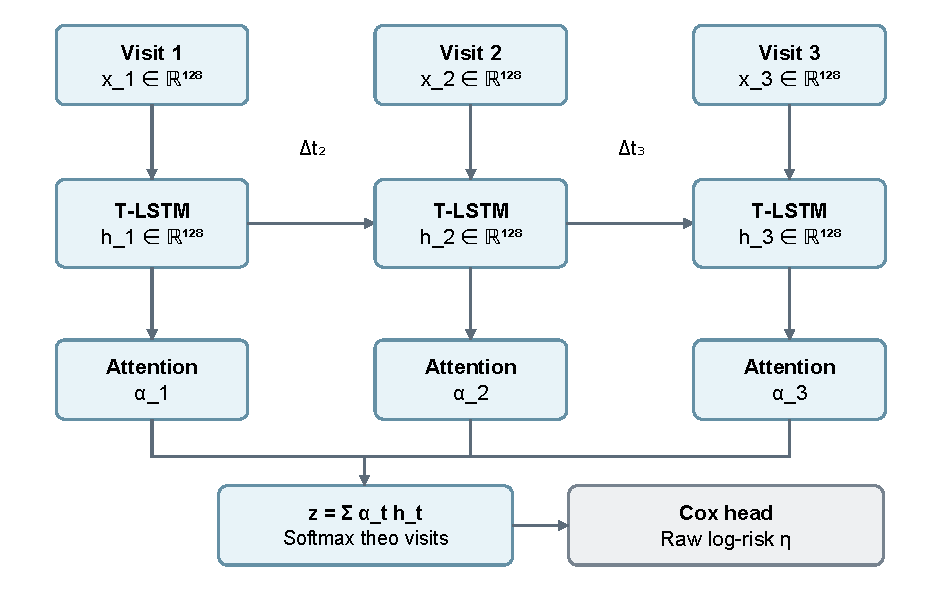
\includegraphics[width=\textwidth]{image/temporal-model.pdf}
\caption[T-LSTM và temporal attention]{Ba visit embeddings và khoảng cách MRI đi qua T-LSTM. Mỗi hidden state được chấm điểm bởi additive attention; tổng có trọng số tạo subject representation cho Cox head. Visit mask điều khiển temporal aggregation, khác với masks cho từng giá trị clinical.}
\label{fig:temporal}
\end{figure}

Masked additive attention lấy cảm hứng từ cơ chế chấm điểm học được \cite{bahdanau2015attention}:
\begin{equation}
 e_t=v_a^\top\tanh(W_a h_t+b_a),\qquad
 \alpha_t=\frac{\exp(e_t)}{\sum_{j\in\mathcal V}\exp(e_j)},\qquad
 z=\sum_{t\in\mathcal V}\alpha_t h_t.
 \label{eq:temporal-attention}
\end{equation}
$\mathcal V$ là tập visits hợp lệ. Attention projection dùng $128\to64\to1$, và $z\in\mathbb R^{128}$. Temporal weights phản ánh cách tổng hợp chuỗi của mạng, không phải mức quan trọng lâm sàng đã được xác nhận của từng visit.

\FloatBarrier
\section{Cox objective, huấn luyện và lựa chọn mô hình}
\label{sec:training-method}
Survival head dùng Linear $128\to64$, GELU, Dropout 0.30 và Linear $64\to1$ để sinh raw log-risk $\eta_i$. Không đặt sigmoid hoặc softmax cuối head. Với giả định proportional hazards \cite{cox1972regression},
\begin{equation}
 h(\tau\mid z_i)=h_0(\tau)\exp(\eta_i).
\end{equation}
Điểm nguy cơ lớn hơn tương ứng nguy cơ event sớm hơn; nó không trực tiếp là xác suất tiến triển ở một horizon cụ thể.

Gọi $\tau_k$ là các event times khác nhau, $\mathcal D_k$ là nhóm events tại $\tau_k$, $d_k=|\mathcal D_k|$ và $\mathcal R_k=\{j:t_j\geq\tau_k\}$. Negative partial log-likelihood với Breslow ties \cite{breslow1974covariance}, trung bình trên số events $N_e$, là
\begin{equation}
 \mathcal L_{\rm Cox}=-\frac{1}{N_e}\sum_k
 \left[\sum_{i\in\mathcal D_k}\eta_i
 -d_k\log\!\left(\sum_{j\in\mathcal R_k}\exp(\eta_j)\right)\right].
 \label{eq:cox-method}
\end{equation}
Trong training thực tế, $\mathcal R_k$ chỉ gồm bệnh nhân trong \emph{physical minibatch}, nên đây là xấp xỉ risk set toàn training cohort. Gradient accumulation không ghép các risk sets thành full-cohort likelihood. Validation loss được tính trên toàn bộ 54 người. Cox arithmetic dùng FP32 và log-sum-exp để giữ ổn định số học.

Protocol chính dùng AdamW \cite{loshchilov2019adamw} với learning rate $10^{-4}$, weight decay $10^{-4}$, betas $(0.9,0.999)$. Physical batch gồm 6 người, tích lũy gradient hai bước; sampling có xét event, không replacement hoặc oversampling. Mô hình dùng AMP FP16, clipping norm 1.0 và tối đa 100 epochs. ReduceLROnPlateau theo full-validation Cox loss dùng factor 0.5, patience 5 và learning rate tối thiểu $10^{-6}$. Early stopping theo validation C-index có warm-up 10 epochs, patience 20 và min-delta 0.002. Best checkpoint được lưu theo validation C-index \cite{harrell1996multivariable}; các run giữ checkpoint cuối để audit trajectory.

Ba seeds 20260727, 20260728 và 20260729 thay đổi khởi tạo, sampling và optimization trên cùng split cố định. Architecture selection sử dụng validation, kiểm tra nhiều seed và standardized validation benchmark; không dùng historical test metrics làm tiêu chí lựa chọn. Formal held-out final evaluation chưa được thực hiện trong phase đánh giá cuối. Kết luận về hiệu năng ở Chương~\ref{chap:results} vì vậy là bằng chứng validation trong cohort và protocol đã mô tả.

\chapter{Thực nghiệm, kết quả và phân tích}
\label{chap:results}

Chương này đối chiếu các mô hình từ MRI một thời điểm, MRI dọc theo thời gian đến các cách hợp nhất thông tin, sau đó dùng ablation để xác định những thành phần cần giữ trong kiến trúc cuối. Kết quả validation được dùng để chọn mô hình; kết quả test hậu nghiệm giúp mô tả hiệu năng của checkpoint đã chọn. RC-Free Pairwise Fusion được giữ làm kiến trúc chính vì có validation cao nhất ở phép so sánh cùng seed và chỉ cần hai cặp tương tác.

\section{Giao thức thực nghiệm và cách đọc kết quả}
\label{sec:experimental-protocol}
Cohort đóng băng gồm 359 người và 1.077 lượt khám, đúng ba visit cho mỗi người. Split theo người bệnh gồm 251 người train, 54 người validation và 54 người test, với 74, 16 và 16 biến cố tương ứng. Chuẩn hóa và PCA chỉ được fit trên train, rồi áp dụng các artifact đã đóng băng cho validation và test. Đầu ra là raw risk; giá trị lớn hơn biểu thị nguy cơ chuyển đổi sớm hơn.

Các bảng một seed sử dụng seed 20260727 và các checkpoint được chọn theo validation trước khi khóa cấu hình để đánh giá test, theo báo cáo đánh giá từ máy chủ. Các bảng ghi epoch của checkpoint được chọn, không phải tổng số epoch huấn luyện. Chỉ số là Harrell-style C-index: người có biến cố được so với người có thời gian theo dõi dài hơn, risk bằng nhau nhận 0,5 điểm và thời gian bằng nhau không tạo cặp so sánh \cite{harrell1996multivariable}. Validation có 480 cặp hợp lệ, còn test có 528 cặp. C-index càng cao càng tốt, được ký hiệu bằng $\uparrow$; ô in đậm là giá trị cao nhất của từng cột Val hoặc Test trong bảng.

Tập test đã từng được truy cập trong quá trình nghiên cứu, vì vậy toàn bộ cột Test trong chương này là \emph{test hậu nghiệm}. Chúng không được dùng để chọn kiến trúc và không được xem là đánh giá độc lập cuối cùng. Benchmark ba seed ở Mục~\ref{sec:standardized-benchmark} chỉ báo cáo validation; trung bình ba seed và một điểm test của seed 20260727 là hai loại bằng chứng khác nhau. Báo cáo test mới được lưu cùng nguồn số liệu, còn các dự đoán từng người và checkpoint trên máy chủ chưa được kiểm tra lại tại môi trường biên soạn.

Với họ MedicalNet Pairwise, CP Pairwise và RC-Free Pairwise, giao thức chính dùng AdamW, learning rate $10^{-4}$, weight decay $10^{-4}$, FP16 AMP, clipping norm 1 và tối đa 100 epoch \cite{loshchilov2019adamw}. ReduceLROnPlateau theo Cox loss toàn validation; early stopping theo C-index dùng warmup 10 epoch, patience 20 và min-delta 0,002. Cox loss xử lý biến cố đồng thời bằng Breslow \cite{cox1972regression,breslow1974covariance}. Risk set lúc train là minibatch vật lý; tích lũy gradient không ghép chúng thành risk set toàn cohort.

\begin{table}[htbp]
\centering
\small
\caption[Giao thức của các nhóm mô hình]{Các nhóm giao thức trong tiến trình phát triển mô hình. Cùng seed và split chưa có nghĩa là mọi cấu hình huấn luyện đều giống nhau.}
\label{tab:protocol-groups}
\begin{tabularx}{\linewidth}{@{}Y C{1.7cm} L{5.3cm}@{}}
\toprule
\textbf{Nhóm mô hình} & \textbf{Cox batch} & \textbf{Phạm vi so sánh} \\
\midrule
MRI Only; Longitudinal MRI & 6 & Khảo sát biểu diễn MRI và thời gian \\
Simple Multimodal Fusion & 8 & Mốc phát triển bằng ghép nối \\
Dynamic/MedicalNet Pairwise & 6 & So sánh initialization có kiểm soát \\
CP/RC-Free Pairwise & 6 & So sánh trong cùng họ pairwise \\
Ablation của CP Pairwise & 6 & Chỉ thay một thành phần so với CP đầy đủ \\
CNN--PCA--T-LSTM Adaptation & 16 & Pipeline tham chiếu, tối ưu riêng trên train \\
\bottomrule
\end{tabularx}
\end{table}

\section{MRI một thời điểm và MRI dọc theo thời gian}
\label{sec:mri-baselines}
\label{sec:longitudinal-results}
MRI Only dùng MRI tại visit cuối để dự báo nguy cơ. Trong so sánh 3D ResNet-18 cùng seed, Random ResNet đạt validation 0,787500, cao hơn MedicalNet 0,733333, nhưng test hậu nghiệm của MedicalNet lại cao hơn. Sự đảo thứ hạng này cho thấy không nên chọn initialization bằng cách nhìn lại test. CrossFormer3D, được thích nghi từ hướng CrossFormer \cite{wang2022crossformer}, giảm số tham số MRI Only từ 33.051.969 xuống 9.856.501 và đạt validation 0,764583; đây là một hướng khảo sát backbone gọn hơn.

\begin{table}[htbp]
\centering
\small
\setlength{\tabcolsep}{4pt}
\caption[C-index của các mô hình MRI trên cùng seed]{MRI một thời điểm và MRI dọc ở seed 20260727. Val/Test là C-index; Test là đánh giá hậu nghiệm. Dấu sao chỉ run attention còn hạn chế về hồ sơ hoàn tất.}
\label{tab:mri-milestones}
\begin{tabularx}{\linewidth}{@{}Y r r r@{}}
\toprule
\textbf{Mô hình} & \textbf{Epoch} & \textbf{Val $\uparrow$} & \textbf{Test $\uparrow$} \\
\midrule
MRI Only -- MedicalNet & 3 & 0,733333 & \bestresult{0,623106} \\
MRI Only -- Random ResNet & 19 & \bestresult{0,787500} & 0,496212 \\
MRI Only -- CrossFormer & 8 & 0,764583 & 0,490530 \\
Longitudinal MRI -- T-LSTM & 32 & 0,733333 & 0,492424 \\
Longitudinal MRI + Attention* & 34 & 0,783333 & 0,577652 \\
Longitudinal MRI -- CrossFormer & 25 & 0,725000 & 0,606061 \\
\bottomrule
\end{tabularx}
\end{table}

Longitudinal MRI dùng chung encoder cho ba visit, sau đó đưa chuỗi embedding qua T-LSTM. Phiên bản lấy trạng thái cuối đạt validation 0,733333; bổ sung attention ghi nhận 0,783333. Run attention được sửa sau lỗi AMP overflow, nhưng hồ sơ hoàn tất trong nguồn lịch sử còn hạn chế, nên được đánh dấu sao dù báo cáo đánh giá mới ghi nhận chạy thành công. Longitudinal MRI với CrossFormer đạt 0,725000. Các mốc này chưa chứng minh rằng thêm MRI theo thời gian tự động cải thiện dự báo; cần kiểm tra biểu diễn thời gian trên nhiều seed và điều kiện huấn luyện đồng nhất.

\section{So sánh các cách hợp nhất thông tin}
\label{sec:concat-results}
\label{sec:dynamic-pairwise-results}
Simple Multimodal Fusion ghép các embedding trước T-LSTM, attention và Cox head, đạt validation 0,812500 và test hậu nghiệm 0,723485. Dynamic Pairwise Fusion mô hình hóa MR, MC và RC bằng outer-product sau chiếu giảm chiều, rồi đưa tương tác trở lại từng nhánh qua gate, hệ số $\lambda$ và identity residual; validation tăng lên 0,828125. Tuy nhiên, Cox batch thay đổi từ 8 sang 6, nên mức tăng này là quan sát trong quá trình phát triển, chưa phải ablation chỉ thay cách fusion.

MedicalNet Pairwise Fusion giữ cấu trúc và giao thức của Dynamic Pairwise, chỉ đổi initialization MRI, đạt validation 0,839583. Đây là đối chứng full outer-product dùng cho thí nghiệm CP. Các biến thể CrossFormer được trình bày cùng tên của cơ chế hợp nhất trong Bảng~\ref{tab:fusion-common-seed}; kết quả test của chúng không được dùng để thay đổi lựa chọn kiến trúc sau khi đã chốt theo validation.

\begin{table}[htbp]
\centering
\small
\setlength{\tabcolsep}{4pt}
\caption[C-index của các cách fusion trên cùng seed]{Các cách fusion ở seed 20260727; Test là C-index hậu nghiệm của checkpoint chọn theo validation. Các nhóm khác giao thức không được coi là ablation chỉ thay fusion.}
\label{tab:fusion-common-seed}
\begin{tabularx}{\linewidth}{@{}Y r r r@{}}
\toprule
\textbf{Mô hình} & \textbf{Epoch} & \textbf{Val $\uparrow$} & \textbf{Test $\uparrow$} \\
\midrule
Simple Multimodal Fusion & 29 & 0,812500 & 0,723485 \\
CrossFormer Concatenation & 22 & 0,806250 & 0,876894 \\
Dynamic Pairwise Fusion & 5 & 0,828125 & 0,844697 \\
MedicalNet Pairwise Fusion & 35 & \bestresult{0,839583} & 0,763258 \\
CP Pairwise Fusion & 8 & 0,821875 & \bestresult{0,884470} \\
CrossFormer Static Pairwise & 9 & 0,804167 & 0,861742 \\
CrossFormer Dynamic Pairwise & 8 & 0,825000 & 0,878788 \\
CrossFormer Gated Residual Pairwise & 28 & 0,830208 & 0,867424 \\
\bottomrule
\end{tabularx}
\end{table}

\begin{figure}[htbp]
\centering
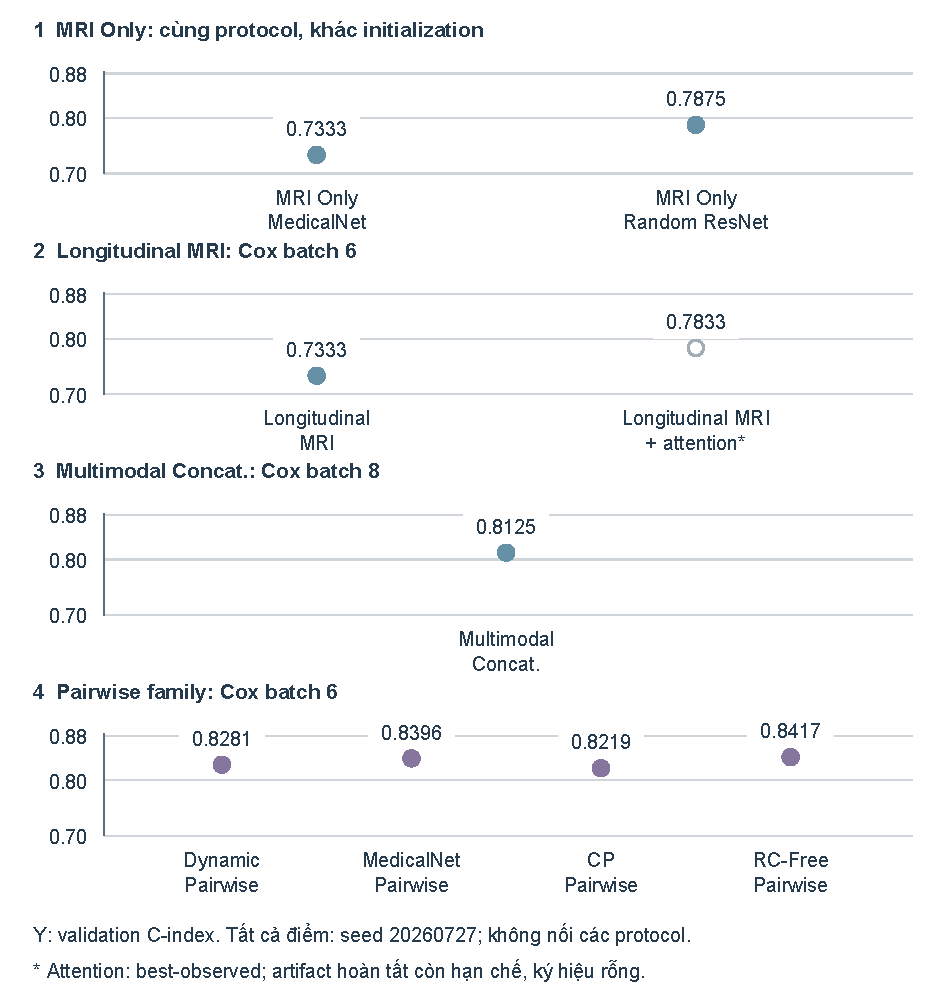
\includegraphics[width=\linewidth]{performance-evolution.pdf}
\caption[Validation theo các nhóm giao thức phát triển]{Các mốc validation ở seed 20260727, tách theo giao thức phát triển. Concatenation dùng Cox batch 8, các nhóm ResNet còn lại dùng batch 6; không nối các nhóm thành một xu hướng tăng điểm có kiểm soát. Dấu sao và marker rỗng chỉ run attention còn hạn chế về hồ sơ hoàn tất. Hình chỉ biểu diễn validation.}
\label{fig:performance-evolution}
\end{figure}

\FloatBarrier
\section{Đối chiếu với CNN--PCA--T-LSTM Adaptation}
\label{sec:paper-adaptation-results}
Kiến trúc tham chiếu của Aghajanian và cộng sự dùng CNN để trích embedding MRI dọc, PCA, T-LSTM và temporal attention cho dự báo sống còn \cite{aghajanian2025longitudinal}. Bản triển khai ở đây được gọi là \emph{CNN--PCA--T-LSTM Adaptation}, vì cohort, tiền xử lý và cấu hình huấn luyện không trùng hoàn toàn với bài báo. Cấu hình T-LSTM được chọn trong train, rồi khóa cho ba seed; validation và test bên ngoài không được dùng trong bước retuning đó.

CNN của từng seed được huấn luyện riêng và cố định để trích embedding 512 chiều trước dropout. PCA99 fit trên train tạo 38, 69 và 2 thành phần cho ba seed; T-LSTM dùng hidden size 64, Adam và batch 16 (Bảng~\ref{tab:alternative-encoder-shapes}). Ở seed 20260727, adaptation đạt validation 0,662500 và test hậu nghiệm 0,537879. Bảng~\ref{tab:baseline-gains} ghi mức tăng C-index so với bản adaptation này; ký hiệu $\uparrow$ thể hiện chiều tốt hơn của chỉ số, không biểu thị ý nghĩa thống kê.

\begin{table}[htbp]
\centering
\small
\setlength{\tabcolsep}{4pt}
\caption[C-index và mức tăng so với CNN--PCA--T-LSTM Adaptation]{C-index và mức tăng so với CNN--PCA--T-LSTM Adaptation trên cùng seed 20260727. Test là hậu nghiệm; mức tăng chỉ áp dụng cho bản adaptation trên cohort hiện tại.}
\label{tab:baseline-gains}
\begin{tabularx}{\linewidth}{@{}Y r r r r@{}}
\toprule
\textbf{Mô hình} & \textbf{Val $\uparrow$} & \textbf{Test $\uparrow$} & \textbf{$\Delta$ Val $\uparrow$} & \textbf{$\Delta$ Test $\uparrow$} \\
\midrule
CNN--PCA--T-LSTM Adaptation & 0,662500 & 0,537879 & $+0{,}000000$ & $+0{,}000000$ \\
MedicalNet Pairwise Fusion & 0,839583 & 0,763258 & $+0{,}177083$ & $+0{,}225379$ \\
CP Pairwise Fusion & 0,821875 & \bestresult{0,884470} & $+0{,}159375$ & $+0{,}346591$ \\
RC-Free Pairwise Fusion & \bestresult{0,841667} & 0,875000 & $+0{,}179167$ & $+0{,}337121$ \\
RC-Free Fixed-$\lambda$ & 0,833333 & 0,850379 & $+0{,}170833$ & $+0{,}312500$ \\
\bottomrule
\end{tabularx}
\end{table}

RC-Free tăng validation 0,179167 và test hậu nghiệm 0,337121 so với adaptation trên split hiện tại. Đây là so sánh giữa hai pipeline có đầu vào và cách huấn luyện khác nhau, nên không thể quy toàn bộ mức tăng cho riêng CP hoặc một route. Bảng cũng không đối chiếu trực tiếp với điểm công bố trên cohort của bài báo gốc.

\section{CP Pairwise Fusion}
\label{sec:cp-results}
CP Pairwise Fusion thay lớp song tuyến đầu tiên của full outer-product bằng $O(A^{\T}x\Had B^{\T}y)+b$. Encoder, post-MLP, directed projection, gate, $\lambda$, residual và mô hình thời gian được giữ nguyên; ranks MR/MC/RC là 8/8/4. CP tham số hóa tensor trọng số, thay vì phân rã dữ liệu của người bệnh.

Ở seed 20260727, CP đạt validation 0,821875 và test hậu nghiệm 0,884470; MedicalNet Pairwise đạt 0,839583 và 0,763258. CP có test cao hơn nhưng validation thấp hơn, nên không thể dùng cột test để tuyên bố CP là lựa chọn tốt hơn. Qua ba seed validation, full outer-product đạt $0{,}834375\pm0{,}014768$, còn CP đạt $0{,}827778\pm0{,}025007$; mean giảm 0,006597. Lợi ích đo được của CP là lõi tương tác ít tham số hơn, trong khi validation vẫn ở mức cạnh tranh.

\section{Ablation: vai trò của từng thành phần fusion}
\label{sec:ablation-results}
Để phân biệt tác động của từng thành phần, ablation lấy CP Pairwise Fusion đầy đủ làm reference và chỉ thay một yếu tố ở seed 20260727. Bỏ gate vẫn giữ $\lambda$ học được; cố định $\lambda=0{,}1$ vẫn giữ gate; bỏ identity residual chỉ bỏ đường truyền trực tiếp embedding gốc. Với biến thể bỏ MR, MC hoặc RC, toàn bộ pair block tương ứng và cả hai route có hướng của cặp đó đều bị bỏ, còn các encoder đầu vào vẫn được giữ.

Độ thay đổi validation so với CP đầy đủ là $\Delta_{\mathrm{Val}}$; chênh lệch giữa hai tập được tính bằng
\begin{equation}
\delta=C_{\mathrm{test}}-C_{\mathrm{validation}}.
\label{eq:split-gap}
\end{equation}
$\delta$ chỉ mô tả hai điểm số của một checkpoint trên hai tập dữ liệu. Giá trị gần 0 không tự chứng minh độ ổn định, bởi hai tập có nhóm người và cặp so sánh khác nhau.

\begin{table}[htbp]
\centering
\small
\setlength{\tabcolsep}{4pt}
\caption[Ablation của CP Pairwise Fusion]{Ablation cùng seed 20260727. Test là C-index hậu nghiệm; $\Delta$ Val so với CP đầy đủ, còn $\delta=\mathrm{Test}-\mathrm{Val}$. Không dùng $\delta$ để chọn mô hình.}
\label{tab:ablation}
\begin{tabularx}{\linewidth}{@{}Y r r r r@{}}
\toprule
\textbf{Biến thể} & \textbf{Val $\uparrow$} & \textbf{Test $\uparrow$} & \textbf{$\Delta$ Val} & \textbf{$\delta$} \\
\midrule
CP Pairwise Fusion & 0,821875 & \bestresult{0,884470} & $+0{,}000000$ & $+0{,}062595$ \\
CP -- Bỏ gate & 0,820833 & 0,867424 & $-0{,}001042$ & $+0{,}046591$ \\
CP -- Cố định $\lambda$ & 0,836458 & 0,862689 & $+0{,}014583$ & $+0{,}026231$ \\
CP -- Bỏ identity residual & 0,827083 & 0,776515 & $+0{,}005208$ & $-0{,}050568$ \\
CP -- Bỏ MR & 0,816667 & 0,842803 & $-0{,}005208$ & $+0{,}026136$ \\
CP -- Bỏ MC & 0,837500 & 0,857008 & $+0{,}015625$ & $+0{,}019508$ \\
RC-Free -- Bỏ RC & \bestresult{0,841667} & 0,875000 & $+0{,}019792$ & $+0{,}033333$ \\
\bottomrule
\end{tabularx}
\end{table}

Trong sáu biến thể thay đổi thành phần, RC-Free có cả validation và test hậu nghiệm cao nhất, lần lượt là 0,841667 và 0,875000. So với CP đầy đủ, validation tăng 0,019792, còn test giảm 0,009470; độ chênh tuyệt đối giữa test và validation giảm từ 0,062595 xuống 0,033333. Như vậy, RC-Free cho sự kết hợp thuận lợi giữa validation cao, test hậu nghiệm cao và cấu trúc ít cặp hơn, nhưng không đạt test cao nhất nếu tính cả reference CP đầy đủ.

\begin{figure}[H]
\centering
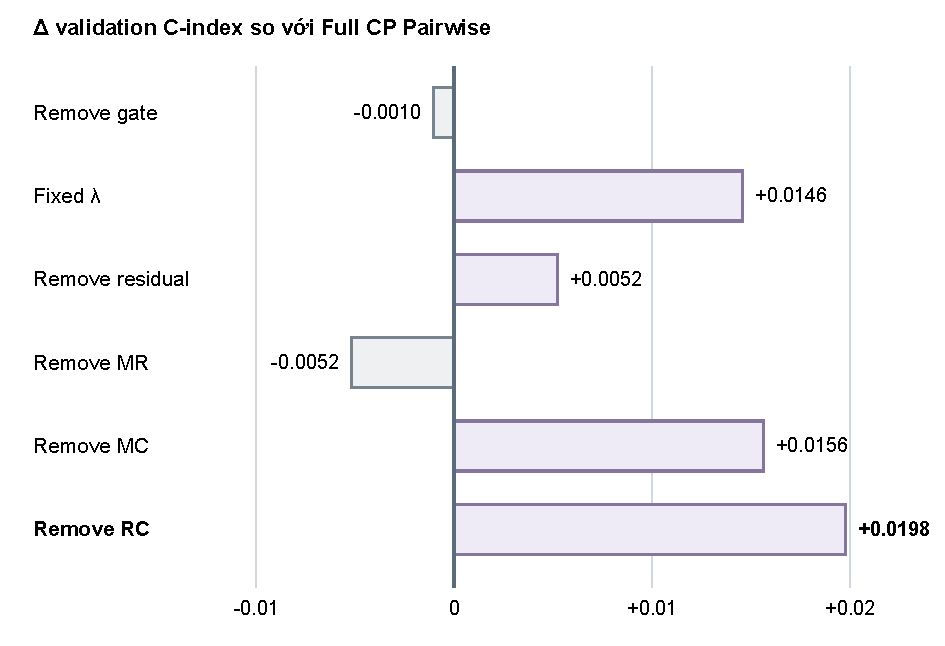
\includegraphics[width=\linewidth]{ablation-deltas.pdf}
\caption[Thay đổi validation trong ablation]{Thay đổi validation C-index so với CP Pairwise Fusion đầy đủ 0,821875 ở seed 20260727. Hình chỉ biểu diễn validation; không có error bar hay kiểm định ý nghĩa thống kê.}
\label{fig:ablations}
\end{figure}

Bỏ MR làm giảm validation, còn bỏ MC và RC làm tăng điểm ở seed này; bỏ identity residual cũng làm test giảm rõ xuống 0,776515. Mức test giảm khi bỏ residual là quan sát hậu nghiệm. Cấu trúc RC-Free được ưu tiên theo validation của ablation và mục tiêu rút gọn tương tác; các số test không được dùng để chọn lại thành phần. Các biến thể cố định $\lambda$, bỏ MR và bỏ MC còn có $|\delta|$ nhỏ hơn RC-Free, vì vậy không dùng riêng chênh lệch test--validation để xếp hạng độ ổn định.

\FloatBarrier
\section{RC-Free Pairwise Fusion và kiểm tra nhiều seed}
\label{sec:rcfree-multiseed}
RC-Free Pairwise Fusion giữ đủ ba nhánh đầu vào, chỉ bỏ cặp RC và hai route $(\mathrm{RC}\to R)$, $(\mathrm{RC}\to C)$. Hai cặp MR/MC, bốn dynamic gate, bốn hệ số $\lambda$ học được, identity residual, T-LSTM và attention được giữ lại. Kiến trúc được chọn theo validation của ablation; test hậu nghiệm dùng để mô tả checkpoint đã chọn.

Validation trung bình ba seed đạt 0,834722 với sample SD 0,023693, cao hơn CP đầy đủ 0,006944 và gần MedicalNet Pairwise, với chênh lệch mean chỉ 0,000347. RC-Free không tốt hơn ở mọi seed: seed 20260729 đạt 0,808333, thấp hơn MedicalNet Pairwise 0,817708. Bằng chứng nhiều seed vì vậy hỗ trợ một cấu trúc gọn có hiệu năng cạnh tranh, thay vì chứng minh ưu thế tuyệt đối.

RC-Free Fixed-$\lambda$ là phép kiểm tra tiếp theo trên cấu trúc chỉ giữ MR/MC; nó khác biến thể cố định $\lambda$ của CP đầy đủ trong bảng ablation. Ở seed 20260727, mô hình này chọn epoch 12, đạt validation 0,833333 và test hậu nghiệm 0,850379. Mean validation ba seed bằng RC-Free, nhưng SD là 0,031273. Việc cố định $\lambda$ chưa tạo ra lợi ích rõ ràng, nên kiến trúc cuối giữ các hệ số học được.

\section{Benchmark validation chuẩn hóa trên ba seed}
\label{sec:standardized-benchmark}
Benchmark đối chiếu các best checkpoint theo ba seed 20260727, 20260728 và 20260729, kiểm tra fingerprint của split, preprocessing train-only và quy ước C-index. Cả 15 ô model--seed được replay từ các run đã tồn tại. Pipeline adaptation vẫn giữ cách huấn luyện riêng; việc chuẩn hóa đánh giá không biến tất cả model family thành một ablation duy nhất.

\begin{table}[htbp]
\centering
\small
\setlength{\tabcolsep}{4pt}
\caption[Benchmark validation chuẩn hóa trên ba seed]{C-index validation chuẩn hóa: mean $\pm$ sample SD ($n=3$). Hai dòng in đậm đồng hạng theo mean. Seed 27/28/29 là 20260727/20260728/20260729.}
\label{tab:standard-bench}
\begin{tabularx}{\linewidth}{@{}Y r r r r@{}}
\toprule
\textbf{Mô hình; C-index $\uparrow$} & \textbf{Seed 27} & \textbf{Seed 28} & \textbf{Seed 29} & \textbf{Mean $\pm$ SD} \\
\midrule
Paper CNN--T-LSTM & 0,662500 & 0,770833 & 0,791667 & $0{,}741667\pm0{,}069347$ \\
MedicalNet Pairwise & 0,839583 & 0,845833 & 0,817708 & $0{,}834375\pm0{,}014768$ \\
CP Pairwise & 0,821875 & 0,855208 & 0,806250 & $0{,}827778\pm0{,}025007$ \\
\bestresult{RC-Free Pairwise} & \bestresult{0,841667} & \bestresult{0,854167} & \bestresult{0,808333} & \bestresult{$0{,}834722\pm0{,}023693$} \\
\bestresult{RC-Free Fixed-$\lambda$} & \bestresult{0,833333} & \bestresult{0,866667} & \bestresult{0,804167} & \bestresult{$0{,}834722\pm0{,}031273$} \\
\bottomrule
\end{tabularx}
\end{table}

Paper CNN--T-LSTM trong bảng là CNN--PCA--T-LSTM Adaptation; MedicalNet Pairwise là full outer-product, CP Pairwise giữ đủ ba cặp, còn RC-Free Pairwise chỉ giữ MR/MC. Hai dòng in đậm đồng hạng theo mean; sample SD dùng mẫu số $n-1$. RC-Free cao hơn adaptation về mean 0,093056, nhưng ba seed dùng cùng split, không phải ba cohort độc lập.

\begin{figure}[H]
\centering
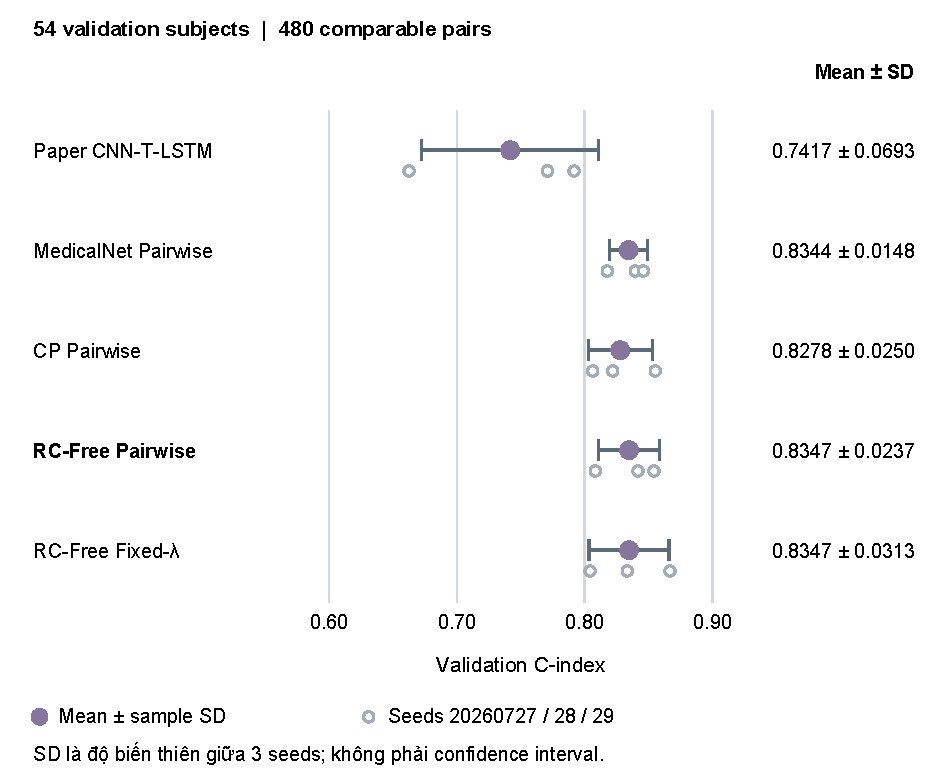
\includegraphics[width=\linewidth]{standardized-benchmark.pdf}
\caption[Benchmark validation chuẩn hóa trên ba seed]{Mean và sample SD validation của năm mô hình. Error bar biểu diễn dao động giữa các seed trên cùng split, không phải khoảng tin cậy hay kết quả test.}
\label{fig:benchmark}
\end{figure}

MedicalNet Pairwise có SD thấp nhất trong nhóm pairwise, còn RC-Free và RC-Free Fixed-$\lambda$ đồng hạng mean. Với chỉ ba seed và nhiều lần dùng validation để chọn kiến trúc, chưa đủ bằng chứng kết luận RC-Free ổn định nhất. Khóa luận chọn RC-Free là cấu hình phù hợp nhất với tiêu chí validation và mục tiêu giữ cấu trúc gọn trong nhóm đã khảo sát.

\FloatBarrier
\section{Hiệu quả về số tham số}
\label{sec:computational-efficiency}
Ba phép biến đổi song tuyến đầu tiên của full outer-product có 229.696 tham số gồm bias. CP giảm chúng còn 3.712, tương đương 98,384\%. Các post-MLP không thay đổi; tính cả post-MLP, tổng của ba pair block giảm từ 248.608 còn 22.624. Bảng~\ref{tab:interaction-parameters} phân biệt lõi interaction với toàn bộ mạng để tránh diễn giải mức giảm 98\% như giảm toàn mô hình.

\begin{table}[htbp]
\centering
\small
\caption[Số tham số của full outer-product và CP]{Số tham số phép biến đổi song tuyến đầu tiên, gồm bias. CP ranks MR/MC/RC là 8/8/4.}
\label{tab:interaction-parameters}
\begin{tabularx}{\linewidth}{@{}Y r r@{}}
\toprule
\textbf{Phạm vi} & \textbf{Full outer-product} & \textbf{CP} \\
\midrule
MR: $32\times32\to128$ & 131.200 & 1.664 \\
MC: $32\times16\to128$ & 65.664 & 1.536 \\
RC: $32\times16\to64$ & 32.832 & 512 \\
\midrule
Tổng ba lớp đầu & 229.696 & 3.712 \\
Ba pair block, gồm post-MLP & 248.608 & 22.624 \\
Toàn mô hình & 33.760.941 & 33.534.957 \\
\bottomrule
\end{tabularx}
\end{table}

\begin{figure}[H]
\centering
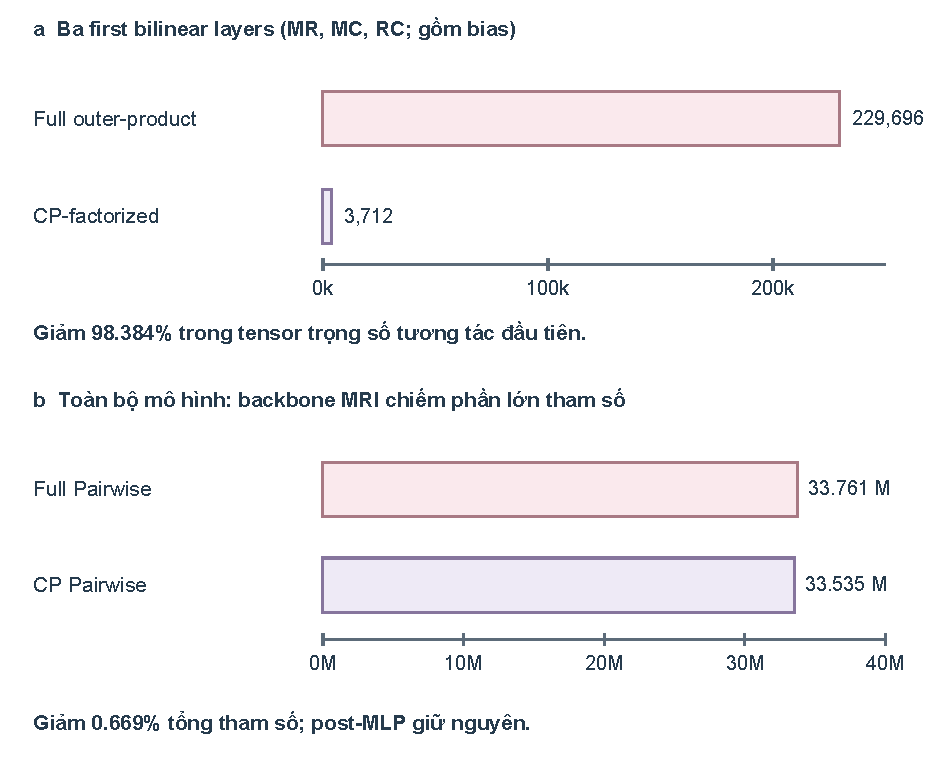
\includegraphics[width=\linewidth]{cp-parameter-reduction.pdf}
\caption[Tham số outer-product và CP theo từng phạm vi]{Giảm tham số từ full outer-product sang CP: 98,384\% ở các lớp song tuyến đầu tiên, nhưng chỉ 0,669\% ở toàn mô hình do MRI encoder chiếm phần lớn tham số. Post-MLP được giữ nguyên.}
\label{fig:cp-parameters}
\end{figure}

RC-Free có tổng 33.519.497 tham số, trong đó hai pair block MR/MC có 19.968 tham số, lõi CP có 3.200, bốn gate có 25.348 và bốn $\lambda$ là bốn scalar học được. Fixed-$\lambda$ còn 33.519.493 tham số. Việc bỏ RC chủ yếu đơn giản hóa interaction graph; mức giảm toàn mạng là nhỏ. Parameter count không thay thế phép đo FLOPs, latency hoặc memory. Các run có số epoch dừng khác nhau nên thời gian train tổng không được dùng như một benchmark tốc độ có kiểm soát.

\FloatBarrier

\section{Kết luận từ thực nghiệm và lựa chọn kiến trúc}
\label{sec:rq-results}
\begin{table}[H]
\centering
\small
\caption[Kết luận cho các câu hỏi nghiên cứu]{Trả lời các câu hỏi nghiên cứu trong phạm vi dữ liệu và giao thức hiện có.}
\label{tab:rq-answer}
\begin{tabularx}{\linewidth}{@{}C{0.9cm}Y@{}}
\toprule
\textbf{RQ} & \textbf{Kết luận và giới hạn} \\
\midrule
RQ1 & Các mốc longitudinal MRI chưa cho thấy lợi ích ổn định so với MRI Only; cần so sánh biểu diễn thời gian trong điều kiện đồng nhất. \\
RQ2 & Simple Multimodal Fusion có validation cao hơn longitudinal MRI, nhưng khác batch và hồ sơ attention hạn chế chưa cho phép tách riêng đóng góp của đầu vào. \\
RQ3 & Pairwise có validation cao hơn concatenation trong tiến trình phát triển; cần đối chứng cùng batch để cô lập tác động của fusion. \\
RQ4 & CP giảm 98,384\% tham số ở các lớp song tuyến đầu tiên; mean validation giảm 0,006597 so với full outer-product. \\
RQ5 & RC-Free có validation cao nhất trong ablation cùng seed, test hậu nghiệm cao và mean validation cạnh tranh qua ba seed; giữ MR/MC là lựa chọn thiết kế được hỗ trợ trong cohort này. \\
\bottomrule
\end{tabularx}
\end{table}

Kiến trúc chính của khóa luận là \textbf{RC-Free Pairwise Fusion}. Quyết định dựa trên validation và mục tiêu đơn giản hóa tương tác; mức test hậu nghiệm 0,875000 bổ sung bằng chứng mô tả, không thay đổi tiêu chí lựa chọn. CP đầy đủ có test cao hơn và MedicalNet Pairwise có SD validation thấp hơn, vì vậy kết luận không mở rộng thành ưu thế trên mọi chỉ số. Đánh giá trên cohort độc lập hoặc một tập giữ lại mới chưa được thực hiện và là bước cần thiết để kiểm chứng khả năng khái quát hóa.

\chapter{Thảo luận, kết luận và hướng phát triển}
\label{chap:discussion}

Các thí nghiệm trong Chương~\ref{chap:results} trả lời một câu hỏi thiết kế cụ thể: có thể khai thác thông tin đa phương thức bằng một interaction graph gọn hơn mà vẫn giữ hiệu năng validation cạnh tranh hay không? Chương này diễn giải các bằng chứng, phân biệt kết luận được hỗ trợ với giả thuyết cần kiểm chứng thêm, và xác định phạm vi sử dụng của mô hình.

\section{Thảo luận}
Kết quả cho thấy dùng ba MRI chưa mang lại lợi ích ổn định so với một MRI. Ghép thêm radiomics và dữ liệu lâm sàng tạo tín hiệu tích cực trên validation, nhưng các giai đoạn còn khác cấu hình huấn luyện nên chưa thể tách riêng lợi ích của từng thành phần. Việc thêm thời điểm hay nguồn thông tin cần được kiểm tra trong cùng điều kiện thí nghiệm.

CP phân rã tensor trọng số của lớp tương tác đầu tiên \cite{kolda2009tensor}, giúp giảm mạnh số tham số của khối này. Trong ba seed, điểm validation trung bình giảm nhẹ so với full outer-product; kết quả chưa cho thấy CP tự cải thiện dự báo. Vì MRI encoder vẫn chiếm phần lớn tham số, mức giảm của toàn mạng nhỏ hơn nhiều. Lợi ích về tốc độ và bộ nhớ cần được đo trực tiếp.

RC-Free được chọn sau ablation một seed và kiểm tra lại bằng ba seed. Mô hình giữ đủ MRI, radiomics và dữ liệu lâm sàng, chỉ bỏ tương tác trực tiếp radiomics--clinical. MRI kết nối với hai nhánh còn lại qua MR và MC (Hình~\ref{fig:mri-hub}); gate điều chỉnh đóng góp theo đầu vào, còn residual giữ thông tin gốc. Kết quả ủng hộ một cấu trúc gọn có hiệu năng validation cạnh tranh trên bộ dữ liệu hiện tại, chưa chứng minh RC vô ích trên mọi dữ liệu. Gate và attention cũng chưa được kiểm chứng như chỉ dấu lâm sàng.

\begin{figure}[htbp]
\centering
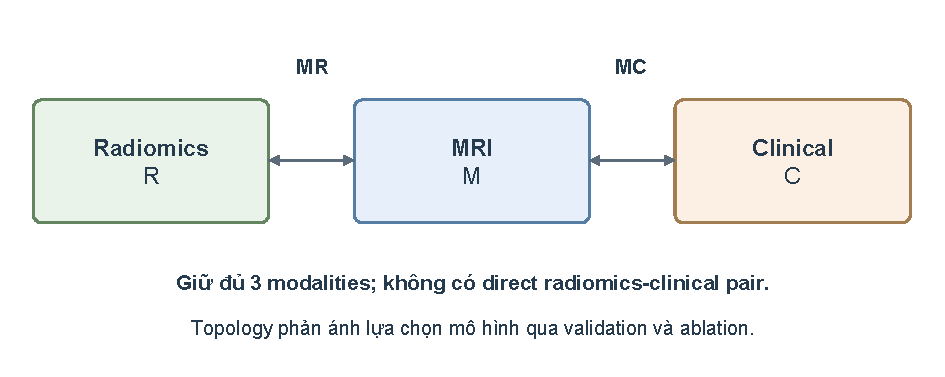
\includegraphics[width=\textwidth]{mri-hub-topology.pdf}
\caption[MRI làm trung tâm của topology RC-Free]{Topology cuối được lựa chọn qua validation và ablation: mô hình giữ đủ MRI, radiomics và clinical, sử dụng MRI làm trung tâm tương tác sau khi bỏ direct radiomics--clinical pair. Các cạnh biểu diễn trao đổi feature qua MR/MC, không phải quan hệ nhân quả hay kết nối giải phẫu.}
\label{fig:mri-hub}
\end{figure}

Cox elastic-net là đối chứng mạnh cho dữ liệu bảng. Tuy nhiên, khác biệt về cách tính C-index và chọn mô hình khiến so sánh với mạng sâu chưa hoàn toàn đồng nhất. Vì vậy, các kết luận chỉ áp dụng trong điều kiện thí nghiệm hiện có.

\section{Giới hạn}
\begin{enumerate}
\item \textbf{Dữ liệu và thời điểm dự báo.} Mẫu nghiên cứu gồm 359 người ADNI có đủ ba MRI trong 18 tháng và không tiến triển sớm. Biến cố dựa trên ngưỡng MMSE/CDR, chưa thay thế chẩn đoán AD được xác nhận. Mốc dự báo là MRI thứ ba, nhưng điều kiện chọn mẫu được kiểm tra đến hết 18 tháng; dữ liệu lâm sàng ghép trong $\pm90$ ngày còn có thể xuất hiện sau MRI. Vì vậy, kết quả chưa chứng minh khả năng dự báo bằng dữ liệu có sẵn đúng tại thời điểm đó.
\item \textbf{Độ chắc chắn của kết quả.} Tập validation chỉ có 54 người và 16 biến cố. Ba seed dùng cùng một phép chia dữ liệu; độ lệch chuẩn giữa seed không phải khoảng tin cậy. Ablation ban đầu chỉ chạy một seed, còn nhiều lần chọn mô hình trên validation có thể làm hiệu năng được đánh giá quá cao. Một số đối chứng khác cấu hình huấn luyện; Cox loss tính trên từng nhóm mẫu (batch) và C-index chỉ đánh giá thứ hạng nguy cơ, chưa đánh giá độ chính xác của xác suất dự báo.
\item \textbf{Kiểm chứng trên dữ liệu mới và hiệu quả triển khai.} Các thí nghiệm trước từng dùng tập test; đánh giá cuối cùng theo quy trình chính thức vẫn chưa được thực hiện. Mô hình chưa được kiểm tra trên nhóm người độc lập, khi thiếu một nguồn dữ liệu hay khi chất lượng MRI thay đổi. Rank CP còn cố định, chưa so sánh nhiều giá trị trong cùng điều kiện huấn luyện. Mức giảm tham số cũng chưa chứng minh mức tiết kiệm thời gian hay bộ nhớ vì chưa có phép đo đồng nhất.
\end{enumerate}

\section{Kết luận}
Khóa luận phát triển một pipeline survival từ MRI-only đến longitudinal MRI, ghép nối đa phương thức, dynamic pairwise fusion, CP-factorized interaction và ablation topology. Quá trình này xuất phát từ câu hỏi của nghiên cứu longitudinal MRI--radiomics: bổ sung một modality bằng ghép nối chưa bảo đảm khai thác được tín hiệu của nó \cite{aghajanian2025longitudinal}.

Kiến trúc được chọn là RC-Free CP-Factorized Pairwise Fusion. Mô hình giữ MRI, radiomics và clinical, tham số hóa MR/MC bằng CP, đưa tương tác trở lại modality qua gated residual, rồi xử lý ba visit bằng T-LSTM và attention trước Cox head. Bằng chứng validation hiện tại ủng hộ một graph gọn có hiệu năng cạnh tranh; CP giảm chi phí của interaction core, còn loại RC đơn giản hóa topology. Các kết luận này là kết luận về thiết kế trong cohort hiện tại, chưa phải xác nhận ưu thế lâm sàng hoặc kết quả test.

\section{Hướng phát triển}
Ưu tiên đầu tiên là xây dựng và đánh giá protocol tiến cứu với time origin rõ ràng, eligibility phù hợp lúc dự báo và clinical chỉ lấy từ các ngày đã quan sát; xác nhận endpoint bằng chẩn đoán có thẩm định nếu có. Cần giữ provenance của dữ liệu hiện tại và tạo phiên bản cohort mới thay vì sửa âm thầm bản đóng băng.

Sau khi khóa protocol, nên thực hiện đối chứng MRI/temporal/modality trên cấu hình đồng nhất, mở rộng số split hoặc cohort độc lập, và chạy formal final evaluation có công bố lịch sử test. Calibration, time-dependent Brier score và các metric theo horizon sẽ bổ sung cho concordance \cite{graf1999brier}. Khoảng tin cậy theo người bệnh cần được tách khỏi SD theo seed.

Các hướng về kiến trúc gồm xử lý thiếu modality, rank-adaptive interaction, uncertainty-aware routing và temporal encoders mới khi quy mô dữ liệu cho phép. Pretrained brain representations như hướng brain latent diffusion có thể hữu ích \cite{li2026longitudinal}, nhưng mọi cải tiến cần được kiểm tra bằng đối chứng phù hợp. Cuối cùng, đo latency, memory và độ ổn định trên phần cứng cố định sẽ làm rõ lợi ích triển khai thực sự của kiến trúc gọn.


\clearpage
\phantomsection
\addcontentsline{toc}{chapter}{TÀI LIỆU THAM KHẢO}
\renewcommand{\bibname}{TÀI LIỆU THAM KHẢO}
\begingroup
\renewcommand{\bibfont}{\normalsize}
\setlength{\bibsep}{2.5pt}
\bibliographystyle{thesisrefs}
\bibliography{references}
\endgroup

\end{document}
